%%%%%%%%%%%%%%%%%%%%%%%%%%%%%%%%%%%%%%%%%
% Wenneker Article
% LaTeX Template
% Version 2.0 (28/2/17)
%
% This template was downloaded from:
% http://www.LaTeXTemplates.com
%
% Authors:
% Vel (vel@LaTeXTemplates.com)
% Frits Wenneker
%
% License:
% CC BY-NC-SA 3.0 (http://creativecommons.org/licenses/by-nc-sa/3.0/)
%
%%%%%%%%%%%%%%%%%%%%%%%%%%%%%%%%%%%%%%%%%

%----------------------------------------------------------------------------------------
%	PACKAGES AND OTHER DOCUMENT CONFIGURATIONS
%----------------------------------------------------------------------------------------

\documentclass[10pt, a4paper, twocolumn]{article} % 10pt font size (11 and 12 also possible), A4 paper (letterpaper for US letter) and two column layout (remove for one column)

%%%%%%%%%%%%%%%%%%%%%%%%%%%%%%%%%%%%%%%%%
% Wenneker Article
% Structure Specification File
% Version 1.0 (28/2/17)
%
% This file originates from:
% http://www.LaTeXTemplates.com
%
% Authors:
% Frits Wenneker
% Vel (vel@LaTeXTemplates.com)
%
% License:
% CC BY-NC-SA 3.0 (http://creativecommons.org/licenses/by-nc-sa/3.0/)
%
%%%%%%%%%%%%%%%%%%%%%%%%%%%%%%%%%%%%%%%%%

%----------------------------------------------------------------------------------------
%	PACKAGES AND OTHER DOCUMENT CONFIGURATIONS
%----------------------------------------------------------------------------------------

\usepackage[english]{babel} % English language hyphenation

\usepackage{microtype} % Better typography

\usepackage{amsmath,amsfonts,amsthm} % Math packages for equations

\usepackage[svgnames]{xcolor} % Enabling colors by their 'svgnames'

\usepackage[hang, small, labelfont=bf, up, textfont=it]{caption} % Custom captions under/above tables and figures

\usepackage{booktabs} % Horizontal rules in tables

\usepackage{lastpage} % Used to determine the number of pages in the document (for "Page X of Total")

\usepackage{graphicx} % Required for adding images

\usepackage{enumitem} % Required for customising lists
\setlist{noitemsep} % Remove spacing between bullet/numbered list elements

\usepackage{multirow}

\usepackage{listings}

\definecolor{dkgreen}{rgb}{0,0.6,0}
\definecolor{gray}{rgb}{0.5,0.5,0.5}
\definecolor{mauve}{rgb}{0.58,0,0.82}  

\lstset{ %
  language=R,                     % the language of the code
  basicstyle=\linespread{1}\ttfamily\footnotesize,       % the size of the fonts that are used for the code
  numbers=left,                   % where to put the line-numbers
  numberstyle=\footnotesize\color{gray},  % the style that is used for the line-numbers
  stepnumber=1,                   % the step between two line-numbers. If it's 1, each line
                                  % will be numbered
  numbersep=5pt,                  % how far the line-numbers are from the code
  backgroundcolor=\color{white},  % choose the background color. You must add \usepackage{color}
  showspaces=false,               % show spaces adding particular underscores
  showstringspaces=false,         % underline spaces within strings
  showtabs=false,                 % show tabs within strings adding particular underscores
  frame=single,                   % adds a frame around the code
  rulecolor=\color{black},        % if not set, the frame-color may be changed on line-breaks within not-black text (e.g. commens (green here))
  tabsize=2,                      % sets default tabsize to 2 spaces
  captionpos=b,                   % sets the caption-position to bottom
  breaklines=true,                % sets automatic line breaking
  breakatwhitespace=false,        % sets if automatic breaks should only happen at whitespace
  title=\lstname,                 % show the filename of files included with \lstinputlisting;
                                  % also try caption instead of title
  keywordstyle=\color{blue},      % keyword style
  commentstyle=\color{dkgreen},   % comment style
  stringstyle=\color{mauve},      % string literal style
  escapeinside={\%*}{*)},         % if you want to add a comment within your code
  morekeywords={*,...}            % if you want to add more keywords to the set
} 

\usepackage{sectsty} % Enables custom section titles
\allsectionsfont{\usefont{OT1}{phv}{b}{n}} % Change the font of all section commands (Helvetica)

%----------------------------------------------------------------------------------------
%	MARGINS AND SPACING
%----------------------------------------------------------------------------------------

\usepackage{geometry} % Required for adjusting page dimensions

\geometry{
	top=1cm, % Top margin
	bottom=1.5cm, % Bottom margin
	left=2cm, % Left margin
	right=2cm, % Right margin
	includehead, % Include space for a header
	includefoot, % Include space for a footer
	%showframe, % Uncomment to show how the type block is set on the page
}

\setlength{\columnsep}{7mm} % Column separation width

%----------------------------------------------------------------------------------------
%	FONTS
%----------------------------------------------------------------------------------------

\usepackage[T1]{fontenc} % Output font encoding for international characters
\usepackage[utf8]{inputenc} % Required for inputting international characters

\usepackage{XCharter} % Use the XCharter font

%----------------------------------------------------------------------------------------
%	HEADERS AND FOOTERS
%----------------------------------------------------------------------------------------

\usepackage{fancyhdr} % Needed to define custom headers/footers
\pagestyle{fancy} % Enables the custom headers/footers

\renewcommand{\headrulewidth}{0.0pt} % No header rule
\renewcommand{\footrulewidth}{0.4pt} % Thin footer rule

\renewcommand{\sectionmark}[1]{\markboth{#1}{}} % Removes the section number from the header when \leftmark is used

%\nouppercase\leftmark % Add this to one of the lines below if you want a section title in the header/footer

% Headers
\lhead{} % Left header
\chead{\textit{\thetitle}} % Center header - currently printing the article title
\rhead{} % Right header

% Footers
\lfoot{} % Left footer
\cfoot{} % Center footer
\rfoot{\footnotesize Page \thepage\ of \pageref{LastPage}} % Right footer, "Page 1 of 2"

\fancypagestyle{firstpage}{ % Page style for the first page with the title
	\fancyhf{}
	\renewcommand{\footrulewidth}{0pt} % Suppress footer rule
}

%----------------------------------------------------------------------------------------
%	TITLE SECTION
%----------------------------------------------------------------------------------------

\newcommand{\authorstyle}[1]{{\large\usefont{OT1}{phv}{b}{n}\color{DarkRed}#1}} % Authors style (Helvetica)

\newcommand{\institution}[1]{{\footnotesize\usefont{OT1}{phv}{m}{sl}\color{Black}#1}} % Institutions style (Helvetica)

\usepackage{titling} % Allows custom title configuration

\newcommand{\HorRule}{\color{DarkGoldenrod}\rule{\linewidth}{1pt}} % Defines the gold horizontal rule around the title

\pretitle{
	\vspace{-30pt} % Move the entire title section up
	\HorRule\vspace{10pt} % Horizontal rule before the title
	\fontsize{32}{36}\usefont{OT1}{phv}{b}{n}\selectfont % Helvetica
	\color{DarkRed} % Text colour for the title and author(s)
}

\posttitle{\par\vskip 15pt} % Whitespace under the title

\preauthor{} % Anything that will appear before \author is printed

\postauthor{ % Anything that will appear after \author is printed
	\vspace{10pt} % Space before the rule
	\par\HorRule % Horizontal rule after the title
	\vspace{20pt} % Space after the title section
}

%----------------------------------------------------------------------------------------
%	ABSTRACT
%----------------------------------------------------------------------------------------

\usepackage{lettrine} % Package to accentuate the first letter of the text (lettrine)
\usepackage{fix-cm}	% Fixes the height of the lettrine

\newcommand{\initial}[1]{ % Defines the command and style for the lettrine
	\lettrine[lines=3,findent=4pt,nindent=0pt]{% Lettrine takes up 3 lines, the text to the right of it is indented 4pt and further indenting of lines 2+ is stopped
		\color{DarkGoldenrod}% Lettrine colour
		{#1}% The letter
	}{}%
}

\usepackage{xstring} % Required for string manipulation

\newcommand{\lettrineabstract}[1]{
	\StrLeft{#1}{1}[\firstletter] % Capture the first letter of the abstract for the lettrine
	\initial{\firstletter}\textbf{\StrGobbleLeft{#1}{1}} % Print the abstract with the first letter as a lettrine and the rest in bold
}

%----------------------------------------------------------------------------------------
%	BIBLIOGRAPHY
%----------------------------------------------------------------------------------------

\usepackage[backend=bibtex,style=authoryear,natbib=true]{biblatex} % Use the bibtex backend with the authoryear citation style (which resembles APA)

\addbibresource{example.bib} % The filename of the bibliography

\usepackage[autostyle=true]{csquotes} % Required to generate language-dependent quotes in the bibliography
 % Specifies the document structure and loads requires packages

%----------------------------------------------------------------------------------------
%	ARTICLE INFORMATION
%----------------------------------------------------------------------------------------

\title{Pricing Asian Options on Commodities with GARCH Model} % The article title

\author{
	\authorstyle{Lue Shen\textsuperscript{1}, Leheng Chen\textsuperscript{1}, Chu Song\textsuperscript{1} and Jing Qian\textsuperscript{1}} % Authors
	\newline\newline % Space before institutions
	\textsuperscript{1}\institution{Department of Mathematics, the Hong Kong University of Science and Technology, Hong Kong SAR, China}\\ % Institution 1
	}

% Example of a one line author/institution relationship
%\author{\newauthor{John Marston} \newinstitution{Universidad Nacional Autónoma de México, Mexico City, Mexico}}

\date{May 14th, 2019} % Add a date here if you would like one to appear underneath the title block, use \today for the current date, leave empty for no date

%----------------------------------------------------------------------------------------

\begin{document}

\maketitle % Print the title

\thispagestyle{firstpage} % Apply the page style for the first page (no headers and footers)

%----------------------------------------------------------------------------------------
%	ABSTRACT
%----------------------------------------------------------------------------------------

\lettrineabstract{This report studies log return time series for 16 commodities, including energy, agriculture and metals. Basic time series analysis, i.e. statistics and correlation analysis, are conducted for all commodity series. Binomial tree method, Monte Carlo simulations with log-normal assumptions and Monte Carlo simulations with GJR-GARCH model are introduced to price Asian options on crude oil, ethanol, natural gas, gold and silver. Multiple conclusions are derived based on the pricing results. Future work is also discussed at the end of this report.}

%----------------------------------------------------------------------------------------
%	ARTICLE CONTENTS
%----------------------------------------------------------------------------------------

\section{Introduction}

Asian option, also called average value option, is essentially an exotic option, whose payoff depends on the path of the underlying price. As presented in equation \ref{eq:1}, the payoff is determined by the strike price and the average underlying price (either arithmetic or geometric) during the option’s life at the maturity. This averaging feature makes it popular among derivative traders, because the payoff will not be affected dramatically from unpredictable oscillations caused by the underlying’s market performance close to maturity, and these kinds of options also provide a nice hedging choice to companies exposed to average prices, say oil production firms and farm producers. Most common underlying for Asian option are commodities and foreign exchange rate. In this report, Asian options on commodities with high liquidity will be utilized to construct numerical examples and examine proposed pricing methods.

\begin{equation} \label{eq:1}
\begin{aligned}
C_T &= (A_T(t,T) - K)^+
\\
P_T &= (K - A_T(t,T))^+
\end{aligned}
\end{equation}

Since their invention in late seventies, several pricing methods have been proposed, and generally speaking, they can be classified into three categories: semi-analytical, approximation and Monte Carlo. The semi-analytical pricing approach assumes the underlying price following a geometric Brownian motion (GBM). Taking logarithms, the average value of the GBM can be expressed in terms of the sum of normal random variables. Using fast Fourier transform (FFT) and convolutions, the final payoff can be calculated in an analytical way. \citep{carverhill1990average} Benhamou applied the same method for discrete Asian options on underlying with non-normal returns in 2000. \citep{benhamou2000fast} Approximation methods approximate the real distribution of the average underlying price at the maturity with tractable ones, such as Edgeworth series expansion \citep{turnbull1991quick} and lognormal distributions \citep{levy1992pricing}. The Monte Carlo approach is a combination of stochastic models and Monte Carlo simulations. Kemna and Vorst proposed a Monte Carlo simulation scheme for the arithmetic average, as well as a variance reduction technique in their paper \citep{kemna1990pricing}.

This report introduces an innovative Monte Carlo scheme to price a discretely monitored Asian options (average value options) on commodities by assuming that log returns of the underlying price follow GJR-GARCH model. Other non-GARCH models, i.e. binomial tree model and Monte Carlo simulations with constant volatility, are also implemented as a comparison to the proposed pricing method.

\section{Theory}

\subsection{Commodities}

A commodity, such as crude oil or wheat, is a basic good used in commerce that is interchangeable with other commodities of the same type. Commodities can be classified into a few categories according to their usages and values, say raw materials, basic resources, agricultural, and mining products, etc. The price of a commodity good is typically determined as a function of its market as a whole: established physical commodities possess actively traded spot and derivative markets.

Commodity futures are agreements to buy or sell a raw material at a specific date in the future at a particular price. The intrinsic value of one commodity future, at any time t during its life, can be expressed by equation \ref{eq:3}. Since its intrinsic value is a linear function of its underlying price and the value of the contract is zero, we assume that the future price is also a linear function of the underlying price with a coefficient close to 1 and it contains all the volatility and underlying price information for us to price their options. Due to data source limitations, prices of commodities are not available to us, hence we study their future prices as an alternative data source for underlying prices, regardless of its minor delays.

\begin{equation} \label{eq:3}
F_t = S_t - f_t
\end{equation}

In this project, 16 commodities from 3 broad categories, namely energy, agriculture and metals, are selected for analysis. For each of them, price data of the most liquid/major future contract is collected for analysis. Details as follow:

\textbf{Energy:}
\begin{itemize}
\item Crude Oil: WTI Financial Futures
\item Natural Gas: Henry Hub Natural Gas Futures
\item Refined Products: RBOB Gasonline Futures
\item Biofuels: Chicago Ethanol (Platts) Futures
\item Coal: Coal (API2) CIF ARA (ARGUS-McCloskey) Futures
\end{itemize}

\textbf{Agriculture:}
\begin{itemize}
\item Corns: Corns Futures
\item Wheats: Chicago SRW Wheat Futures
\item Soybean: Soybean Futures
\item Soybean Meal: Soybean Meal Futures
\item Soybean Oil: Soybean Oil Futures
\item Livestock: Live Cattle Futures
\item Livestock: Lean Hog Futures
\end{itemize}

\textbf{Metals:}
\begin{itemize}
\item Gold: Gold Futures
\item Silver: Silver Futures
\item Platinum: Platinum Futures
\item Copper: Copper Futures
\end{itemize}


\subsection{Asian Options}

Asian option, also named average value option, is one of the most popular path dependent options among derivative traders. Its payoff is determined by the average underlying price over some pre-set period of time. The average price of the underlying asset can either determine the underlying settlement price or the option strike price. This is different from the case of usual European options and American options, whose payoff depends on underlying price at the exercise date. Hence Asian option is a typical form of exotic options. These exotic features provide risk reduction of market manipulation of the underlying instrument close to maturity \citep{kemna1990pricing}. On top of that, the cost of Asian options is usually much lower than European or American options with same strike and maturity.

Suppose $S_t$ is the underlying price at time $t$, $A_T(0, T)$ is the arithmetic average underlying price at maturity $T$, then we have

\[ A_T(0,T) = \frac 1T \sum_{t=0}^T S_t \]

in discrete form, or in continuous form like this

\[ A_T(0,T) = \frac 1T \int_0^T S_t dt\]

For geometric average underlying price, say $\tilde{A}_T(0, T)$, can be expressed as
\[ \tilde{A}_T(0, T) = (\prod_{t=0}^T S_t )^{\frac 1T}\]

in discrete form, or in continuous form like this

\[ \tilde{A}_T(0, T) = \exp (\frac 1T \int_0^T \log S_t dt) \]

For a European Asian call or put option with strike price $K$, its payoff becomes

\[ C_T = (A_T(0,T) - K)^+\]

or

\[ P_T = (K - A_T(0,T))^+\]

In this report, only arithmetic average underlying price in discrete form is taken into considerations for final payoff. We use strike prices and maturities from 5 commodity option contracts to construct numerical examples, say European Asian call/put options, for proposed pricing models. Considering different specifications, there are 319 option contracts in total, with maturity varying from 5 days to 5 years. Their contract specifications, together with latest settlement prices, are collected as reference. Here is the list:

\begin{itemize}
\item WTI Crude Oil Asian Option
\item Chicago Ethanol (Platts) Asian Option
\item Gold American Option
\item Silver American Option
\item Natural Gas European Option
\end{itemize}

\subsection{Forward Risk Free Interest Rates}
In any pricing model based on numerical methods, the risk free rate always plays an important part and will affect the final pricing results significantly. Since all of the interested options as well as their underlyings are traded in US exchanges,  US treasury yield curve on the day we collect price data will be regarded as risk free rate in numerical models. To implement risk free rate and simulate movements of underlying prices, the forward curve can be constructed as the following:

\begin{equation} \label{eq:4}
\begin{aligned}
f(t_i, t_{i+1}) &= \frac {\log (e^{r_{t_{i+1}}t_{i+1}} / e^ {r_{t_i}t_i)}} {t_{i+1} - t_i}
\\
&= \frac {r_{t_{i+1}}t_{i+1} - r_{t_i}t_i}{t_{i+1} - t_i}
\end{aligned}
\end{equation}

In equation \ref{eq:4}, $r_{t_i}$ is the yield of a treasury instrument maturing at $t_i$, and it can be regarded as the risk free rate for $(0,t_i)$. $f(t_i, t_{i+1})$ is the forward rate in $(t_i, t_{i+1})$ derived by two treasury instruments with adjacent maturity dates.

\subsection{Asian Option Pricing Models}

\subsubsection{Binomial Tree Model}

The binomial tree model uses tree structure to simulate the path of the underlying asset over the whole life of Asian option and applies the forward shooting grid method to avoid the exponential growth of average price. In this case, we add extra grids to record the possible average price and restrict the number of possible average price to be linear growth. To update the average value when the asset value jumps, we use gird function to determine the updated average price.

Under Black-Scholes world, we assume that the volatility of asset value is constant. For the binomial tree, let the jump factor $ u, d $ to be $ u=\exp(\sigma\sqrt{\Delta t}), d=\exp(-\sigma\sqrt{\Delta t}) $ where $ \sigma $ is constant volatility, and $ \Delta t $ is the time step. 

Denote $ S^n_j $ and $ A^n_k $ to be the asset value jumping upward $ j $ times and average price with index $ k $ at $ n $-th time level, respectively. To restrict the possible values for $ F $ to a certain set of predetermined values, we limit the number of averaging values to some multiple of the number of values assumed by the asset price: Assume the coefficient to be $ 1 / \rho \in \mathbb{N} $. For a given time step $ \Delta t $, we let the asset value $ S^n_j $ and the average value $ A^n_k $ to be:
\begin{equation}
\begin{split}
&S^n_j= S_0 e^{j \Delta W}, \ \ A^n_k = S_0 e^{k \Delta Y}, \\ &\Delta W = \sigma\sqrt{\Delta t},\ \Delta Y = \rho\Delta W j, k \in\mathbb{N}
\end{split}
\end{equation}

Then consider at $ (n, j) $ node, for a upward jump from $ (n, j) $ to $ (n + 1, j + 1) $, the asset price will change from $ S^n_j $ to $ S^{n + 1}_{j + 1} $. Let $ A^{n + 1}_{k^+(j)} $ to be the updated value changing from $ A^n_k $ by the upward move. Then by usual computation of updating average value, we have:
\begin{equation}\label{arith: avg}
A^{n + 1}_{k^\pm(j)} = \frac{(n + 1) A^n_k + S^{n +1}_{j \pm 1}}{n + 2}
\end{equation}
Note that $ A^{n + 1}_{k^{\pm}(j)} $ do not coincide with $ A^{n + 1}_{k'} = S_0 e^{k' \Delta Y} $ for some $ k' \in \mathbb{N} $ in general, indicating that $ k^\pm(j) $ may not be integer. Recall $ A^{n + 1}_{k^{\pm}(j)} = S_0 e^{k^{\pm}(j) \Delta Y} $ and $ S^{n + 1}_{j \pm 1} = S_0 e^{(j \ pm 1) \Delta W} $, by \eqref{arith: avg}, we equate the two parts and have the grid function:
\begin{equation}\label{arith: grid func}
k^{\pm}(j) = \frac{\ln\frac{(n + 1) \exp(k \Delta Y) + \exp((j \pm 1) \Delta W)}{n + 2}}{\Delta Y}
\end{equation}

Let $ K' $ denote a subset of integer s.t. $ A^{n + 1}_{k'} \leq A^{n + 1}_{k^{\pm}(j)} $ Define $ k^{\pm}_{floor} $ s.t. $ A^{n + 1}_{k^{\pm}_{floor}} = \max_{k' \in K'} S^{n + 1}_{k'} $. In other words, $ k^{\pm}_{floor} = \lfloor k^{\pm}(j) \rfloor $, then $ k^\pm_{ceil} = k^\pm_{floor} + 1 $. Define $ k_{floor} = \lfloor k \rfloor $ and $ k_{ceil} = k_{floor} + 1 $. At $ n $th step, we have $ A_t \in [-S^n_n, S^n_n] $ and thus $ -n/\rho \leq k \leq n/\rho $. This helps us to restrict the size of $ k $. For a $ k \leq | S^n_n | $, we have $ A^n_k \in [A^n_{floor}, A^n_{ceil}] $ and $ -n/\rho \leq k_{floor} < k_{ceil} \leq n/\rho $ at $ n $th time step.

To solve the problem that that $ k^\pm(j) $ may not be integer, we define the linear interpolation formula that will be used in our FSG method.

Let $ c^n_{j, l} $ denote the numerical approximation to the Asian call value at $ (n, j) $ node with the averaging state variable assuming the value $ A^n_l $. Similar notations for $ c^n_{j, l_{floor}} $ and $ c^n_{j, l_{ceil}} $. For $ j \in \mathbb{R} / \mathbb{N} $, the $ c^n_{j, l} $ will be approximated by linear interpolation:
\begin{equation}\label{arith: interpolation}
c^n_{j, l} = c^n_{j, l_{floor}} + \varepsilon_l (c^n_{j, l_{ceil}} - c^n_{j, l_{floor}})
\end{equation}
where $ \varepsilon_l $ is the fraction of one step $ \Delta Y $ between $ \ln A^n_{l_{ceil}} $ and $ A^n_{l_{floor}} $:
\begin{equation}
\varepsilon_l = \frac{\ln\frac{A^n_l}{A^n_{l_{floor}}}}{\Delta Y}, A^n_l =  A^n_{l_{floor}} e^{\varepsilon_l \Delta Y}
\end{equation}

Finally we have the pricing formula under a binomial tree schemes is given by:
\begin{equation}\label{arith: back induction}
\begin{split}
c^n_{j, k} &= \frac{1}{R} \left[ p c^{n + 1}_{j + 1, k^+(j)} + (1 - p) c^{n + 1}_{j - 1, k^-(j)}\right] \\
&\approx \frac{1}{R} \{ p \left[ \varepsilon_{k^+(j)} c^{n + 1}_{j + 1, k^+_{ceil}} + (1 - \varepsilon_{k^+(j)}) c^{n + 1}_{j + 1, k^+_{floor}} \right] \\
&+ (1 - p) \left[ \varepsilon_{k^-(j)} c^{n + 1}_{j - 1, k^-_{ceil}} + (1 - \varepsilon_{k^-(j)}) c^{n + 1}_{j - 1, k^-_{floor}} \right]\} \\
&n = N - 1, \cdots, 0, j = -n, -n + 2, \cdots, n, \\
&k \in \mathbb{N} \cap [-\frac{n}{p}, \frac{n}{p}]
\end{split} 
\end{equation}
where the risk neutral probability of jump upward is :
\begin{equation}
p=\frac{R-d}{u-d}, \ \ R = e^{r_t (T - t)}
\end{equation}
where $ r_t $ is the forward rate at time $ t $, Finally, the terminal payoff of put and call are:
\begin{equation}\label{arith: terminal}
\begin{split}
&p^N_{j, k} = \max(K - S_0 e^{k \Delta Y}, 0) \\
&c^N_{j, k} = \max(S_0 e^{k \Delta Y} - K, 0), \\
&j = -N, -N + 2, \cdots, N
\end{split}
\end{equation}

\subsubsection{Monte Carlo Simulations with Constant Volatility}

In this method, the underlying commodity price $S_t$ is assumed to follow the stochastic process below:

\begin{equation} \label {eq:5}
dS_t = (r_t - \frac 12 \sigma^2)S_t dt + \sigma S_t dW_t
\end{equation}

where $W_t$ is a standard Wiener process, $r_t$ is the risk free interest rate at time $t$, $\sigma$ is a constant, representing the volatility of the underlying price's log return.

With US treasury yield curve, the forward the rate at time $t$ can be used to represent $r_t$ for simulations, and its calculation method is covered in section 2.3 already. With historical future prices of the commodity's major future contract, the volatility $\sigma$ can be calculated as

\begin{equation} \label{eq:6}
\begin{aligned}
r_i &= \log S_{t_i} - \log S_{t_{i-1}}
\\
\sigma &= \sqrt {\frac 1{N-1} \sum_{i=1}^N (r_i - \bar r)^2}
\end{aligned}
\end{equation}

Given a commodity start price $S_0$, the underlying price movements can be simulated by the dynamics of its log returns $\{r_i\}$:

\begin{equation} \label{eq:mcpricing}
\begin{aligned}
dS_t &= (r_t - \frac 12 \sigma^2)S_t dt + \sigma S_t dW_t
\\
d\log S_t &= (r_t - \frac 12 \sigma^2) dt + \sigma dW_t
\\
r_i &= r_{i-1} + (r_t - \frac 12 \sigma^2) dt + \sigma dW_t
\\
S_{t_i} &=S_{t_{i-1}}\exp(r_i \Delta t) = S_0\exp(\sum_{k=0}^i r_k \Delta t)
\end{aligned}
\end{equation}

The average price $A_T(0,T)$ at the maturity is essentially

\[ A_T(0,T) = \frac 1N \sum_{i=0}^N S_{t_i}\]

where $t_0 = 0$, $t_N = T$.

Without loss of generality, Asian call option is used to illustrate the Monte Carlo scheme, and the put option can be easily derived thereafter. The Asian call option payoff becomes

\[ V_T = (A_T(0,T) - K)^+\]

With $n$ paths of simulated underling prices, the fair payoff at the maturity can be expressed as an average of the payoff generated from each path.

\[\bar V_T = \frac 1n \sum_{i=1}^n V_T^i \]

Multiplying with corresponding discount factor, the value of the contract at present can be derived.

\begin{equation}
\begin{aligned}
df(0,T) &= \exp (-\sum_{i=0}^{N-1} r_{t_i}\Delta t)
\\
\bar V_0 &= df(0,T) \bar V_T
\end{aligned}
\end{equation}

where $r_{t_i}$ is the forward risk free interest rate at $t_i$, and $\Delta t = 1/252$.

Since the underlying is only traded on business days, BUS/BUS date convention is implemented in the simulation scheme.

\subsubsection{Monte Carlo Simulations with GJR-GARCH model}

As a comparison to the constant volatility MC scheme, GJR-GARCH model defines the log return of underlying price as a GARCH process. For a given time series $\{ S_t\}$,

\begin{equation}
\begin{aligned}
r_t &= \log S_t - \log S_{t-1}
\\
r_t &= \mu +\epsilon_t
\\
\epsilon_t &= \sigma_t Z_t
\end{aligned}
\end{equation}

where $Z_t$ follows a standard normal distribution and

\begin{equation}
\begin{aligned}
\sigma_t^2 &= \omega + \sum_i {\alpha_i \epsilon_{t-i}^2} + \sum_j {\beta_j \sigma_{t-j}^2}  \\
&+ \sum_k {\gamma_k \epsilon_{t-k}^2 I_{\epsilon_{t-k} < 0}}
\end{aligned}
\end{equation}

This model will illustrate the volatility behavior of the time series, and since the volatility is the source engine to generate simulated price paths, we assume that a more subtle volatility model will contribute to more accurate pricing results.

In this report, for each commodity, the best model configuration, say the number of $\alpha$, $\beta$, $\gamma$ and whether using zero mean, is selected based on the following steps.

\textbf{Step one: zero mean vs constant mean}

Constant mean model will be considered at the first place. If the p-value of $\mu$ is larger than 0.05, then the mean is considered as insignificant, and it will be removed to refit the model again as a consequence.

\textbf {Step two: Ljung-Box test}

The fitted model will be plugged into historical data, and the series of $\{ Z_t\}$ is derived. If $\{ Z_t\}$ passes Ljung-Box test at a significance level of 0.05, then it proves that the model well explains the historical time series. Otherwise, the model will be rejected.

\textbf {Step three: BIC}

Bayesian information criterion (BIC) is implemented as a criterion for model selection, instead of Akaike information criterion (AIC). This is because BIC has more punishments on number of parameters when the data set is large comparing AIC. 

\begin{equation}
\begin{aligned}
AIC &= 2k - 2\ln (\hat L)
\\
BIC &= \ln(n) k - 2\ln (\hat L)
\end{aligned}
\end{equation}

where $\hat L$ is the maximized value of the likelihood function of the model, $k$ is the number of parameters of the model to estimate, and $n$ is the sample size.

If one model has a less BIC and less number of parameters than the other one, it will be selected as the temporary best model. Alternatively, if BIC of one model is $5\%$ less than the other one, it will also win the selection.

With the best fitted GJR-GARCH model, the volatility of future log returns will be predicted. A series of $\{ \sigma_0(t)\}$ can be derived, since

\[ \sigma_0(t) = E_0[\sigma(t)]\]

and then a path of underlying price can be derived from the generated log return series ${r_t}$, where

\[r_t = \mu + \sigma_0(t) Z_t\]

The rest pricing procedure is the same as the constant volatility scheme.

\section{Process}

\subsection{Data Source}

There are two types of data involved in this project, say commodity future price and option specifications. All of commodity future price data are retrieved from investing.com, a global financial portal owned by Fusion Media Limited. The time span starts from 2000-01-03 and ends at 2019-03-22. However, some futures, like silver and corn, may not have such a long price history. In this case, we take as earlier as we can, and all the future prices are available after year 2009. On the other hand, the option contract specifications and corresponding latest settle prices are recorded manually from CME group website, and there are 319*2=638 options in total (319 call put pairs).

\subsection{Data Preprocess}

The commodity prices are retrieved one by one, hence to further analyze or utilize them, one must concat price series into one data table with respect to dates. The concatenation generates plenty of missing values due to the difference in trading day conventions. For example, futures of silver, platinum and US soybean oil can be traded on Sundays, and all other future contracts will have missing prices on those days. Besides, the time span also varies from one commodity to another, which produces missing values for those with shorter time span before their first date point.

Two preprocessing rules are developed, one for time series analysis while the other for pricing.

\textbf {Preprocessing for time series analysis:}

When two time series are selected for correlation analysis or collinearity analysis, only date points when both have data will be kept and all the date points with missing values will be removed.

\textbf {Preprocessing for pricing:}

Since Asian options only have one underlying, every historical time series will be handled independently. Thus date points with missing values will be dropped in this case.

For option specification data, the currency unit for strike price is different from each other, some are using USD cent, some are 0.001 USD. A currency divisor dictionary is specially created, and the strike price will all be converted to USD before pricing.

\subsection{Correlation Analysis}

Correlation analysis is a method of statistical evaluation used to study the strength of a relationship between two, numerically measured, continuous variables. In this step, the correlation coefficients among future prices and price log returns are calculated respectively by equation \ref{eq:correlation}. Heat maps are used to reflect their relationships. The results are shown in section 4.1.

\begin{equation} \label{eq:correlation}
\begin{aligned}
\rho_{xy} &= \frac {\sum_{i=1}^n (x_i-\bar x)(y_i-\bar y)}{(n-1)s_xs_y}
\\
&=\frac {\sum_{i=1}^n (x_i-\bar x)(y_i-\bar y)}{\sqrt{\sum_{i=1}^n(x_i - \bar x)^2 \sum_{i=1}^n(y_i - \bar y)^2}}
\end{aligned}
\end{equation}

\subsection{Non-GARCH Model Pricing}

This part illustrates the process of Non-GARCH model pricing.

\subsubsection{Binomial Tree Method}

We use binomial tree model to price the current Asian option value. We first calculate the historical volatility of log return. Then we compute the forward rate based the U.S. treasury yield curve. We will use the historical volatility and forward rate as the volatility and risk free rate of the model. For choosing the time step, we consider the total number of business days from the spot date to maturity date. If the time length reaches over 1 year, we restrict the time steps to 252, so that the computational speed could be faster. Since the underlying asset is futures and each futures contract contains more than one unit of goods, hence we choose the price the option that the underlying asset contains 1 unit good.

\subsubsection{Monte Carlo Simulations}

After data preprocessing, the option specifications are stored in one data table, and the underlying table is stored in the other. To price one option with Monte Carlo simulations, the option specifications are retrieved as strike price $K$, start date $t$, maturity date $T$, and underlying name.

Using the underlying name, the fixed volatility $\sigma$ can be derived from historical underlying price data, as mentioned in section 2. The forward risk free interest rates are also calculated from treasury yield curve before simulations. The step size of Monte Carlo simulation is one business date, so the number of steps can be derived from Julian date difference of $t$ and $T$.

For every simulation, the underlying price path can be generated by following equation \ref{eq:mcpricing}. Then the average price at the maturity, say $A_T(0,T)$ can be calculated based on the prices along the path. And the final discounted final payoff can be derived correspondingly, the average value of which will be the value priced by Monte Carlo simulation method.

\subsection{GARCH Model Pricing}

Before pricing the option, the best GARCH model needs to be selected from 2000 possible models ($2\times10\times10\times10$). There are 10 possible values, say from 0 to 9, for each of $\alpha$, $\beta$ and $\gamma$, and the model can be either zero mean or constant mean. The details about model selection criterion is mentioned in section 2.4.3. With the best fitted GARCH model, predictions for mean of volatilities can be derived from the model. Since the step size is one business day, the number of predictions equal to the number of business days from commercing date  and the maturity of the option.

The rest pricing procedure are the same as those of Monte Carlo simulations mentioned in last section, except for the simulation scheme for underlying prices, which follows in section 2.4.3.

\section{Results}

\subsection{Correlation Results}

The heap maps are shown in the appendices.

Figure \ref{priceCorrelation} is the correlation coefficient heat map of future prices. It is clear that there are many strong positive linear relationships between some contracts, such as crude oil and gasoline or silver and platinum or soybean products. There is almost no strong negative linear relationships, but two commodities, say natural gas and live cattle, are less correlated to all other commodities. Except for those commodities made from same materials and those with competitive relationships, most of correlation coefficients are very high, say close to right color in heat map. These present randomness of correlations in commodity prices.

By contrast, figure \ref{logRtCorrelation} shows the correlation coefficient heat map of future log returns. Strong correlations are only presented between commodities within the same category, especially in agriculture or metals, and the log returns in same category are positively correlated.

\subsection{Model results}

\begin{table}[!ht]
\centering
\small
\begin{tabular}{ccccc}
\toprule
Underlying & $ (\alpha, \gamma, \beta) $ & $ Q(20) $ & p-value & BIC \\
\midrule
Crude Oil WTI & (1,1,1) & 13.69 & 0.84 & 21129 \\
Ethanol & (1,1,1) & 39.91 & 0.005 & 13715 \\
Gold & (1,0,1) & 27.53 & 0.12 & 14403  \\
Natural gas & (1,0,1) & 23.48 & 0.2 & 24608 \\
Silver & (1,0,5) & 29.42 & 0.07 & 12151 \\
\bottomrule
\end{tabular}
\caption{Model result: GJR model for each underlying futures}
\label{model result}
\end{table}

Table \ref{model result} shows the model we fit based on BIC criteria. The p-value of Ljung-Box test shows that the GJR-GARCH model for Crude Oil, Gold, Natural gas and Silver is adequate but the model for Ethanol is not. The order of first four GJR-GARCH models are all lest than 1, indicates that the selected model is simple. The order of the last model(Silver) is (1, 0, 5), indicating that the volatility of Silver contract has long memory compared to other underlying futures.

\paragraph{Convergence of the Monte Carlo simulation} 

Figure \ref{oil conv}, \ref{eth conv}, \ref{silver conv}, \ref{gas conv} shows the sample mean of the  call option payoff on Monte-Carlo simulation, The x-axis shows the simulation times and y-axis shows the estimated option value. These figures shows that the option value convergences to a single value and hence the option value from the Monte-Carlo simulation is rational. The prediction of the volatility is shown in appendix.

For the three pricing model(GARCH-MC, MC, BT), we use the following criterion to evaluate the performance of the model:
 
\paragraph{ARE}

We use ARE to evaluate the difference between market price and fair price derived from the model. The formula of ARE is:
\begin{equation}\label{are}
ARE = \frac{1}{N} \sum^N_{j = 1} \frac{\vert V^{model}_j - V^{market}_j \vert}{V^{market}_j} \times 100
\end{equation}
where $ N $ is the total number of the samples, $ V^{model}_j $ and $ V^{market}_j $ are the fair price from the model and the market price of the $ j $-th sample, respectively. The results are shown in table \ref{are stat} \citep{zhu2015model}.

Compared to market price, GARCH-MC model outperforms to other model when the underlying assets are Ethanol and Silver, and call option on Gold, put option on Crude Oil. The MC model outperform on call option on Crude Oil, put option on Natural gas. The BT model outperforms only on call option on Natural gas. Therefore, the fair price form GARCH-MC model is the closets price to the market price.

\paragraph{Fair price of European option}

Instead of market price, the European option price calculated from BS model can also be used as criterion. The analytical value calculated from the BS formula is also a fair price under BS world. Since Asian option uses the average price of the whole path to compute the payoff while European option only consider the asset price on maturity, the risk of holding one unit of European option should be larger than holding one unit of Asian option. Hence the fair price of the Asian option should be smaller than the European option value with the same specification of options.

Denote $ N_s $ as the total number that the fair price of Asian option is smaller then the corresponding European option with the same specification and $ N $ as the total number of samples. We use the proportion $ PS = N_s / N $ as the statistic to evaluate the model, the result is:
\begin{table}[!ht]
\small
\centering
\begin{tabular}{cccc}
Models & $ PS_{call} $ & $ PS_{put} $ \\
GARCH-MC & 1 & 1 \\
MC & 1 & 1 \\
BT & 1 & 1 \\
\end{tabular}
\caption{Proportion of number of Asian option value smaller than European option value with same specification}
\label{PS}
\end{table}

From table \ref{PS}, we can conclude that all the value from our model are rational.


\section{Discussions}

\subsection{Data Limitations}
Commodity futures are the assessment of raw materials trading in open market. Future prices are essentially estimates for the value of future commodities, instead of the spot price. The difference between two prices, say future price and spot price, will be affected by delivery time, risk-free rate, storage cost and convenience yield. Therefore, it will bring inaccuracies into the pricing process when using futures price not the commodity spot prices.

Besides, only WTI Crude Oil Asian option and Chicago Ethanol (Platts) Asian option are Asian options and all the rest options are either American or European options, specifications of which are used to construct numerical examples for the proposed pricing models. In future studies, more traded Asian options settings should be collected to examine these models.

\subsection{Model Limitations}
Chicago Ethanol (Platinum) futures has many duplicate prices on adjacent dates in the early stage, resulting in zero log returns. Moreover, there is no fitted GJR-GARCH model for it, and GJR-GARCH(1,1,1) is used to fit its time series of log returns. However, ARIMA(0,0,1) can sufficiently explain the time series, we may consider applying ARIMA GARCH to fit the historical data and embedding into Monte Carlo scheme in further studies.

\subsection{Monte Carlo Limitations}

In Monte Carlo GARCH method, although Monte Carlo simulations are executed 10000 times, the standard deviation of payoffs generated is relatively large compared to constant volatility Monte Carlo method. This indicates that the number of paths might not be enough. Hence in GARCH Monte Carlo simulations, the final payoff could be a partial solution, and it may take million paths to obtain an output with lower variance. On top of that, the payoff variance from the proposed GARCH Monte Carlo simulation might underestimate the real variance, especially when the number of simulated path is insufficient. In this case, probability bounds analysis (PBA) can be implemented as an examination for partial information. Using PBA, the sparse simulations will provide far-apart upper and lower bounds, and this will well estimate the risk in pricing results.

\subsection{Advanced GARCH Models}

Affine GARCH model is described as the following:

\begin{equation}
\begin{aligned}
r_t &= r - \frac 12 \sigma_t^2 + \sigma_t Z_t
\\
\sigma_t^2 &= \omega + \alpha_1 (Z_{t-1} -\lambda \sigma_{t-1})^2+\beta_1 \sigma_{t-1}^2
\end{aligned}
\end{equation}

According to Lorenzo, a semi-analytical formula for geometric Asian options can be provided when the underlying follows an affine GARCH process and the extreme asymmetry of this kind of models with non-normal innovations will price more accurately for options with very short time to maturity\citep{lorenzo2011pricing}. Hence, affine GARCH might provides a better pricing result if it is implemented to Monte Carlo simulation scheme.



\section{Conclusions}

In this report, 16 commodity future prices are studied, and 5 options of them are priced by three pricing methods, say binomial tree model, Monte Carlo simulations with constant volatility, and Monte Carlo simulations with GJR-GARCH volatility. Strong sector correlations are discovered in the 16 time series of commodity log returns. According to pricing result analysis, the ARE criterion shows that GJR-GARCH model is the most appropriate pricing model in three models implemented in this report. However, there are also a few limitations in this report, say the data limitations and Monte Carlo convergence limitations. There are also other advanced GARCH models, say affine GARCH, to examine in the future studies.

%----------------------------------------------------------------------------------------
%	BIBLIOGRAPHY
%----------------------------------------------------------------------------------------
\printbibliography[title={References}] % Print the bibliography, section title in curly brackets

%----------------------------------------------------------------------------------------
\onecolumn
\newpage
\section{Appendices}
\subsection{Figures}
\begin{figure}[!ht]
	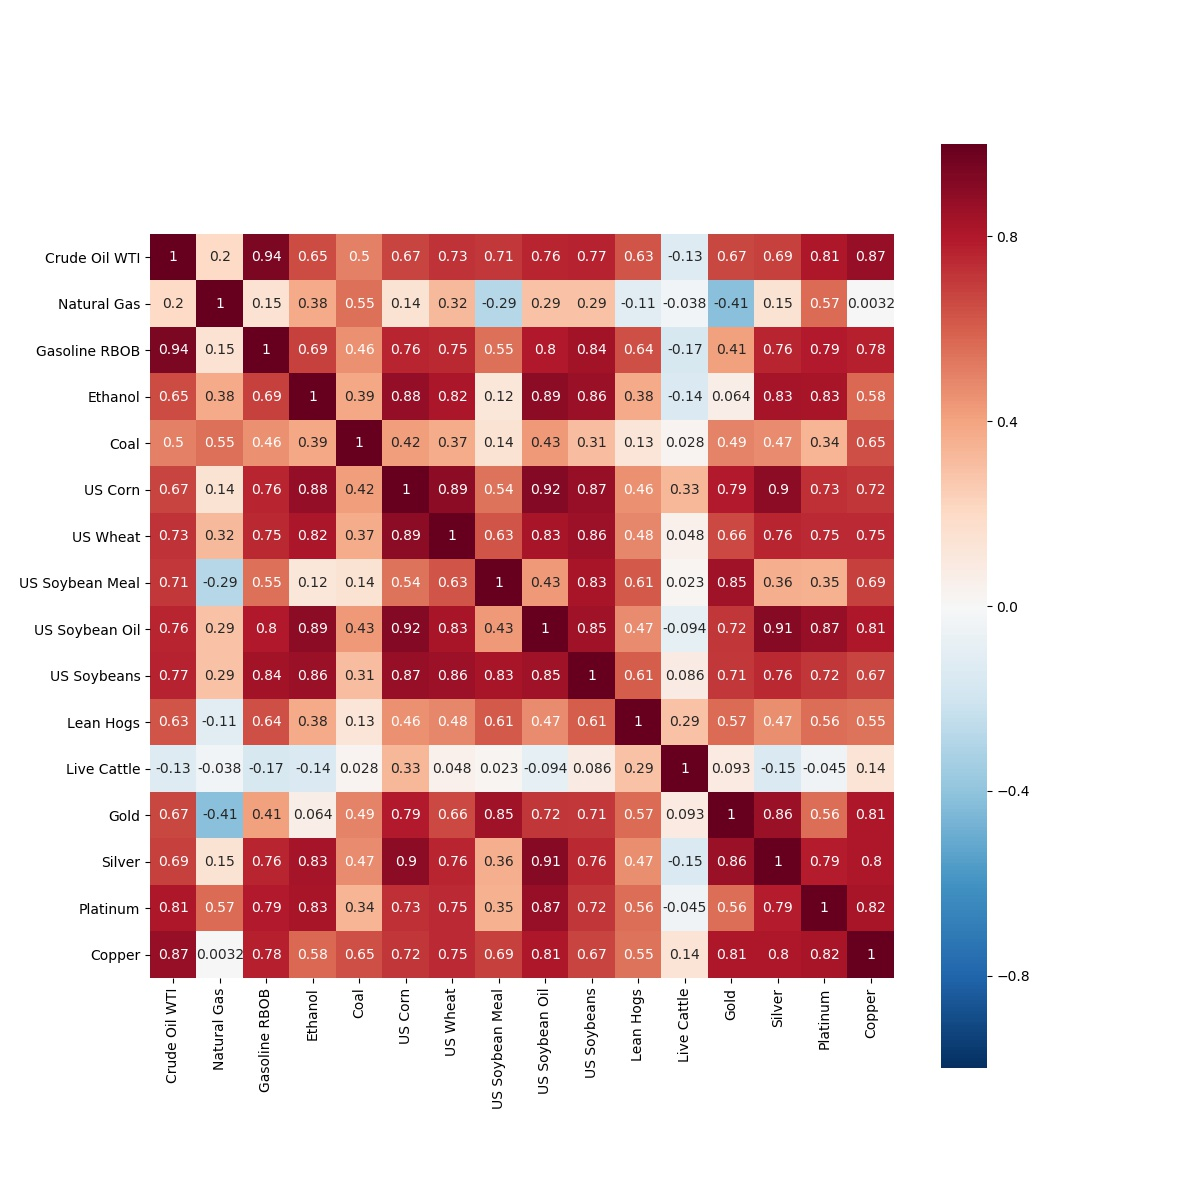
\includegraphics[width=\linewidth]{priceCorrelation.jpg} % Figure image
	\caption{Correlation Analysis of Commodity Prices} % Figure caption
	\label{priceCorrelation} % Label for referencing with \ref{bear}
\end{figure}

\begin{figure} [!ht]
	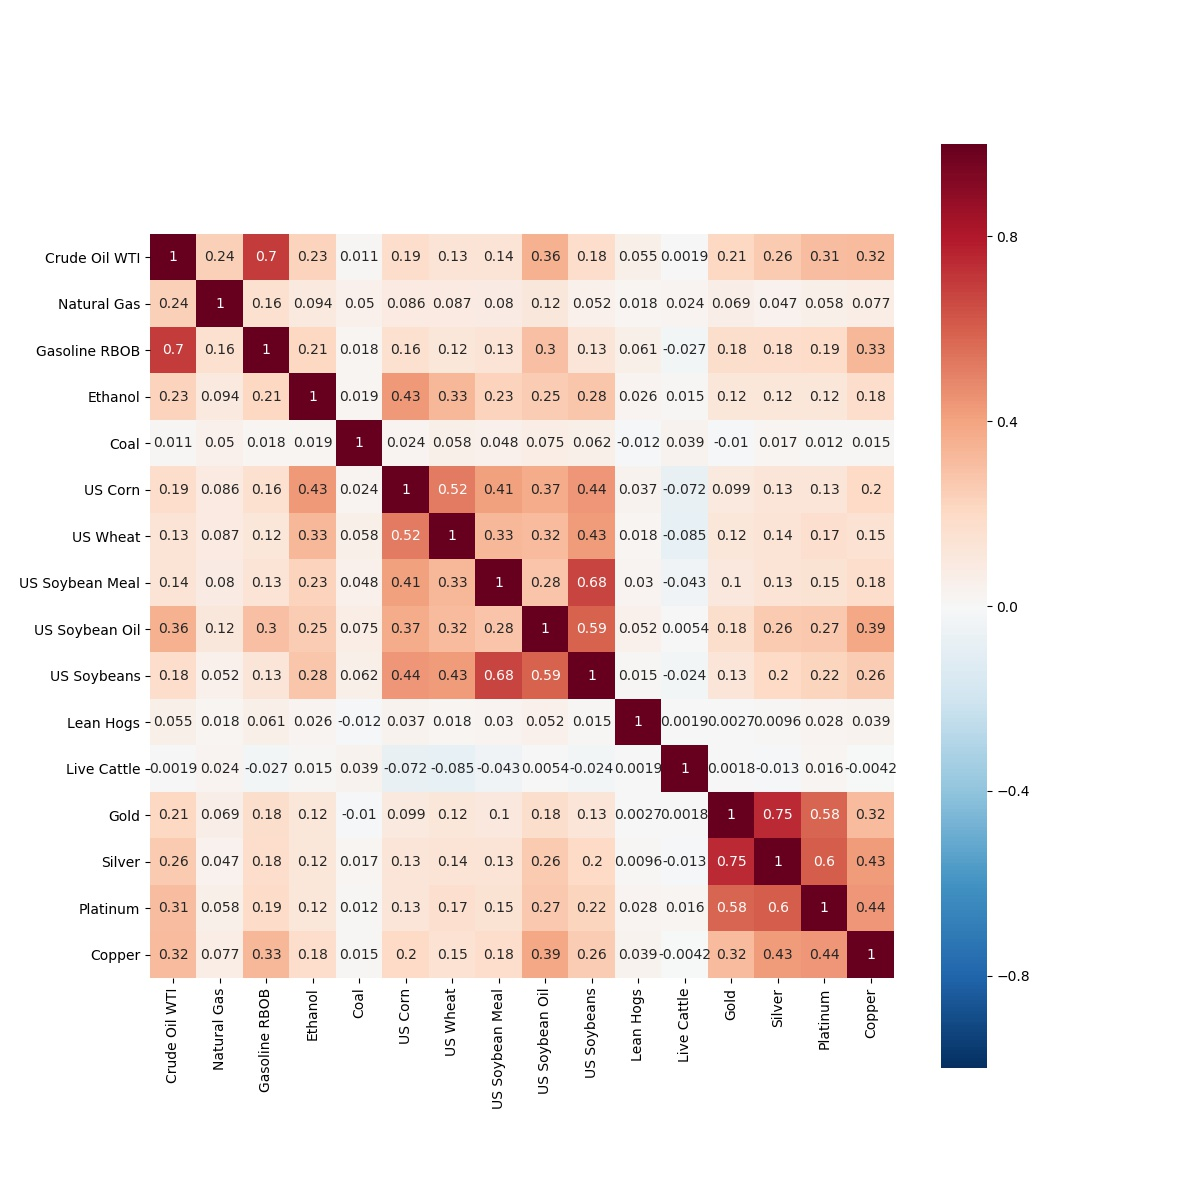
\includegraphics[width=\linewidth]{logRtCorrelation.jpg} % Figure image
	\caption{Correlation Analysis of Commodity Log Returns} % Figure caption
	\label{logRtCorrelation} % Label for referencing with \ref{bear}
\end{figure}

\begin{figure} [!ht]
	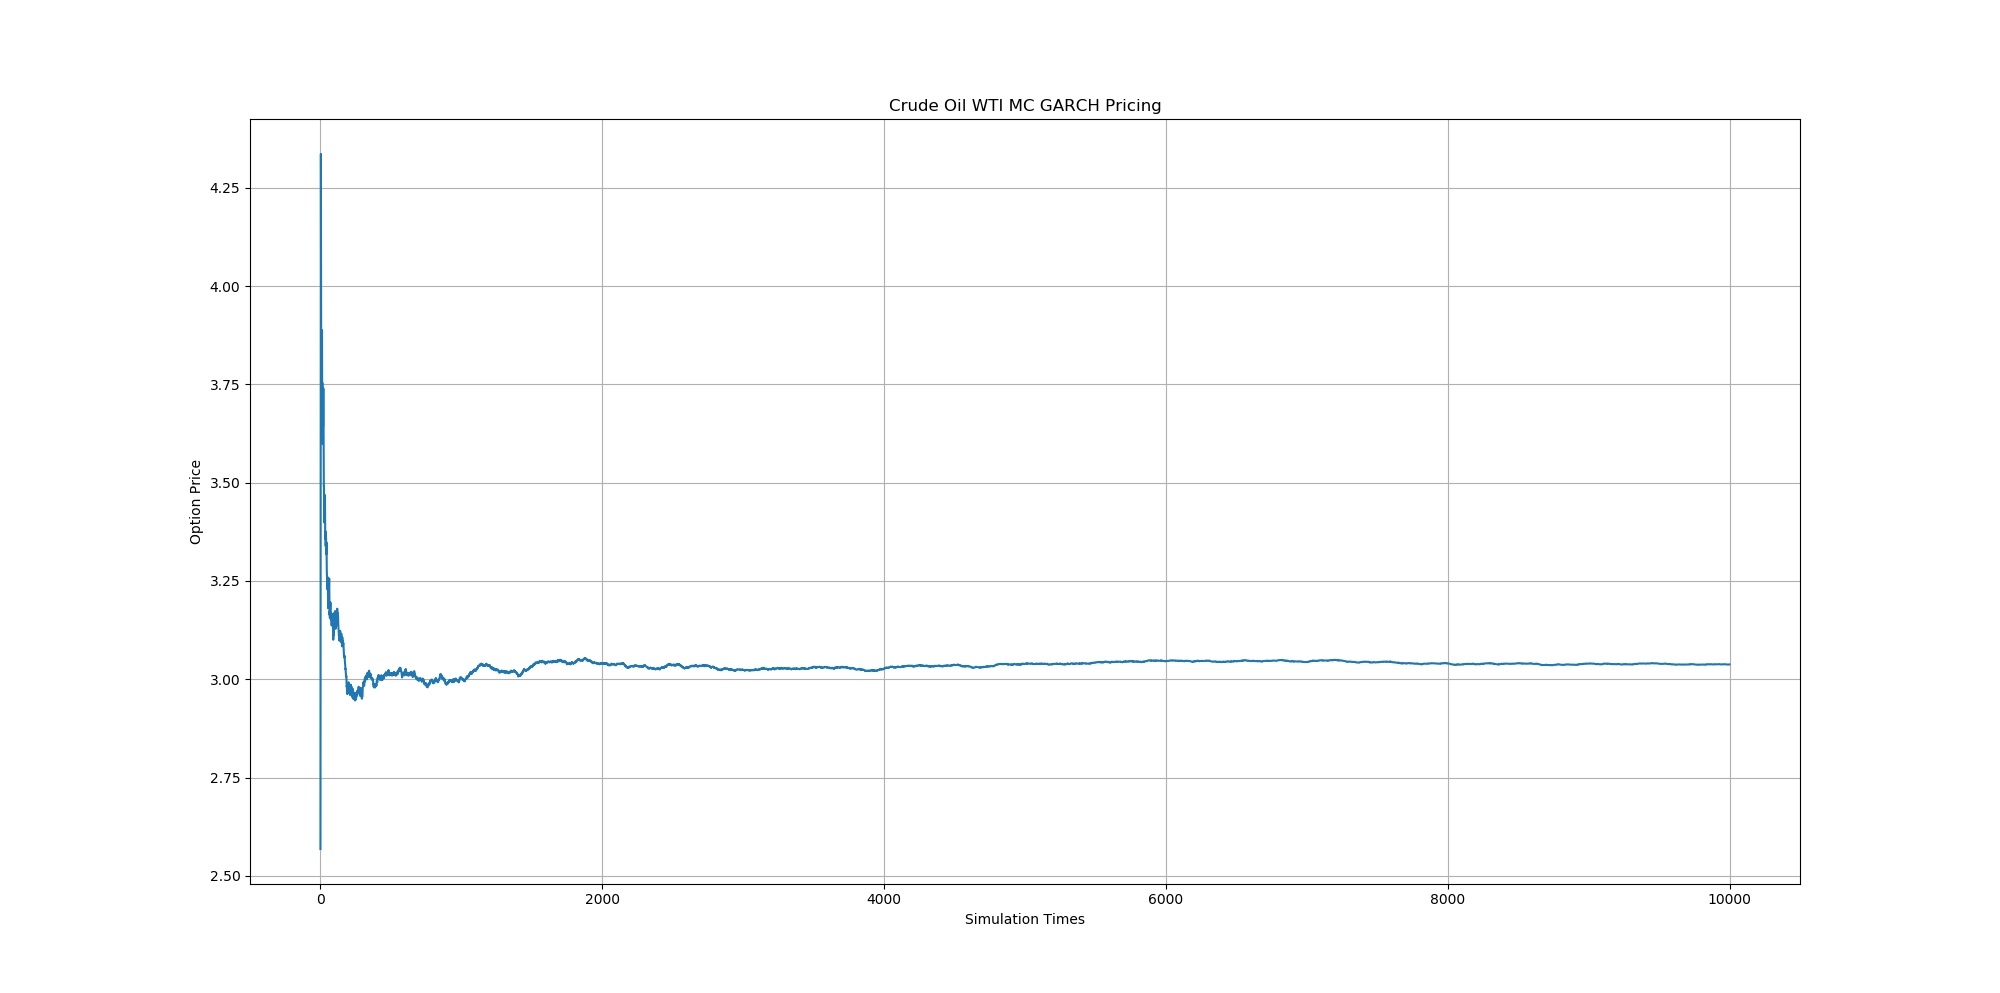
\includegraphics[width=\linewidth]{Curdeoilmcconvergence1.png} % Figure image
	\caption{Convergence Plot for a Crude Oil Asian Option} % Figure caption
	\label{oil conv} % Label for referencing with \ref{bear}
\end{figure}

\begin{figure}[!ht]
	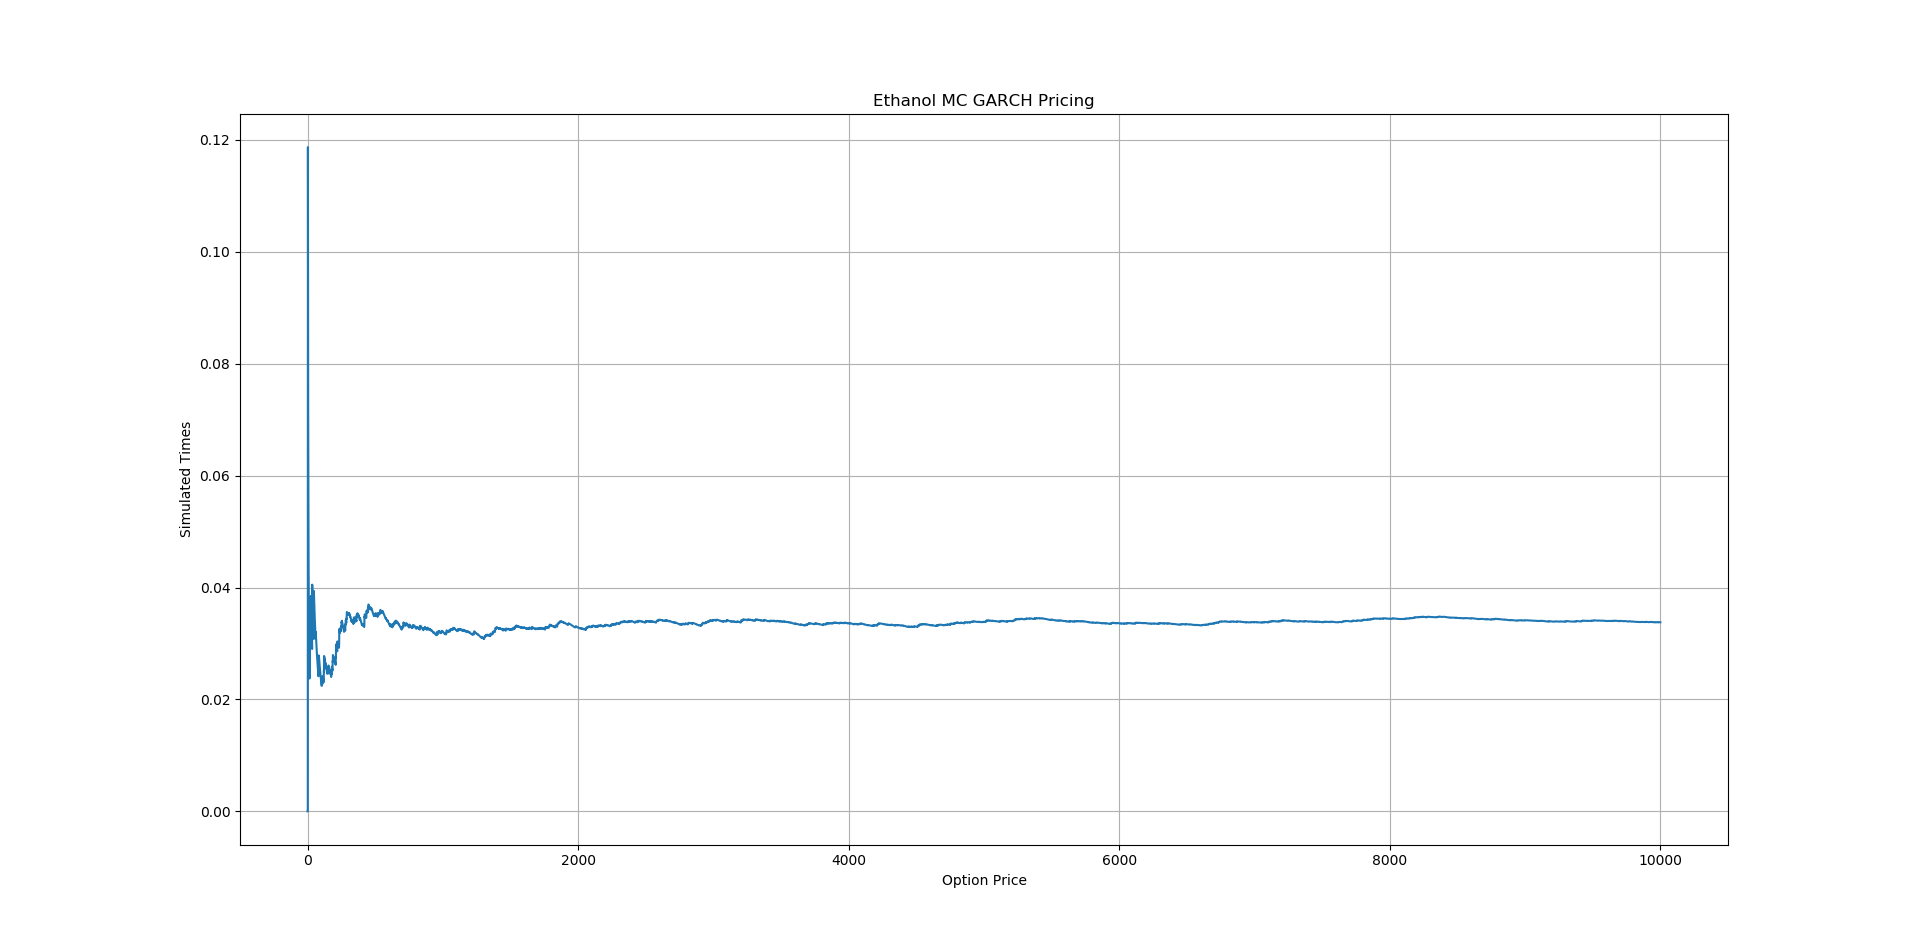
\includegraphics[width=\linewidth]{Ethanolmcconvergence1.png} % Figure image
	\caption{Convergence Plot for an Ethanol Option} % Figure caption
	\label{eth conv} % Label for referencing with \ref{bear}
\end{figure}

\begin{figure}[!ht]
	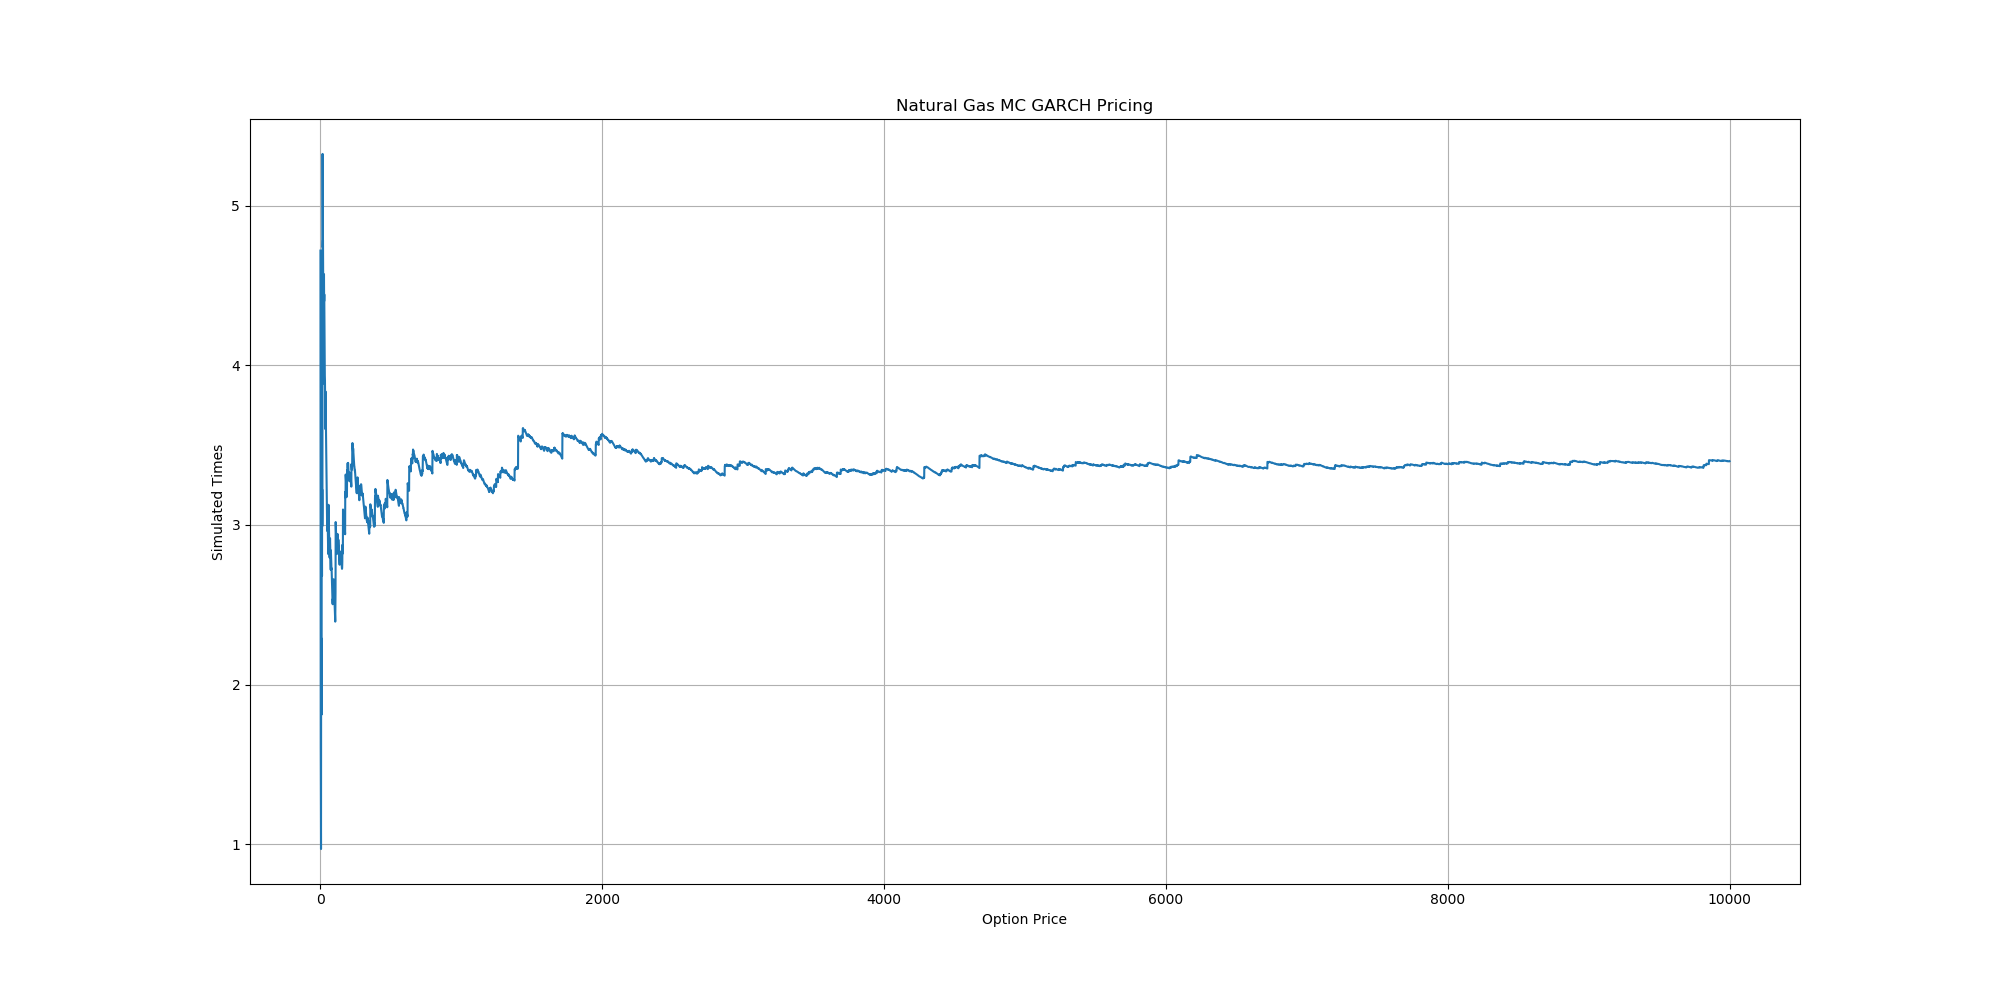
\includegraphics[width=\linewidth]{Naturalgasmcconvergence1.png} % Figure image
	\caption{Convergence Plot for a Natural Gas Asian Option} % Figure caption
	\label{gas conv} % Label for referencing with \ref{bear}
\end{figure}

\begin{figure}[!ht]
	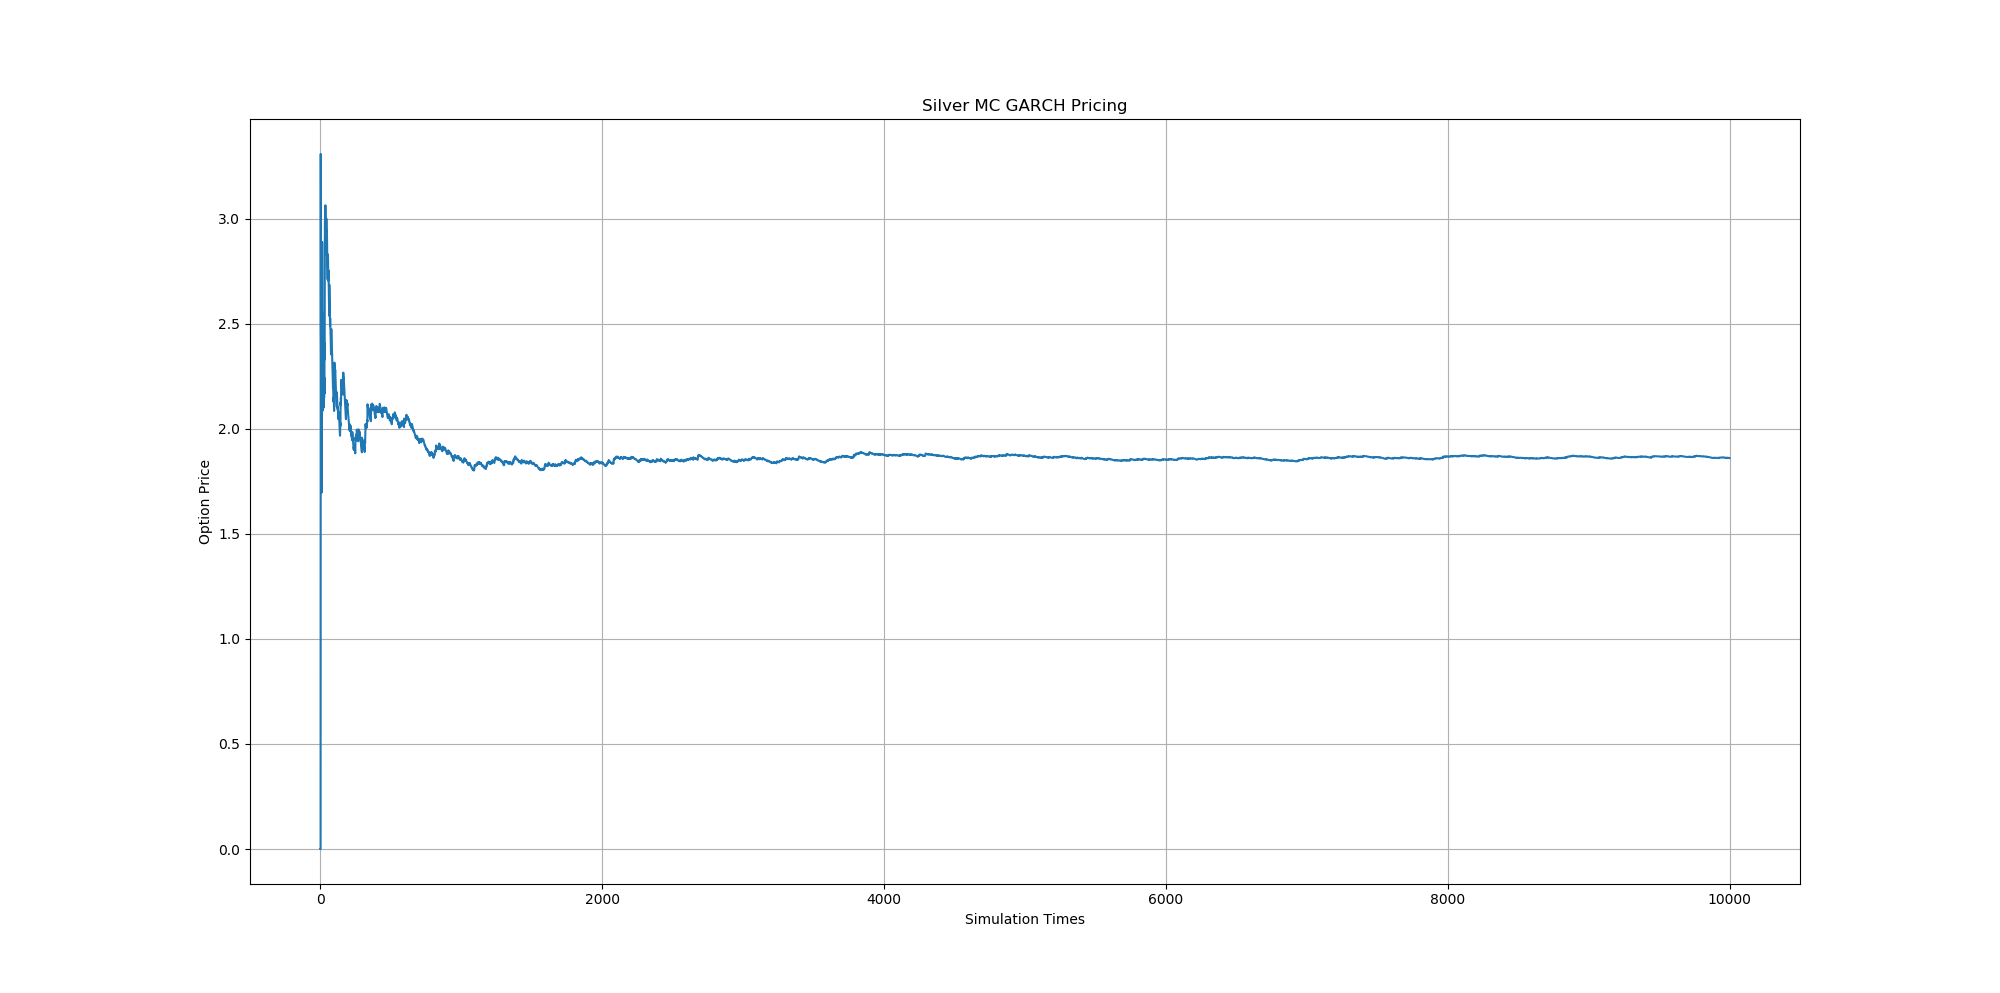
\includegraphics[width=\linewidth]{Silvermcconvergence1.png} % Figure image
	\caption{Convergence Plot for a Silver Asian Option} % Figure caption
	\label{silver conv} % Label for referencing with \ref{bear}
\end{figure}

\begin{figure}[!ht]
	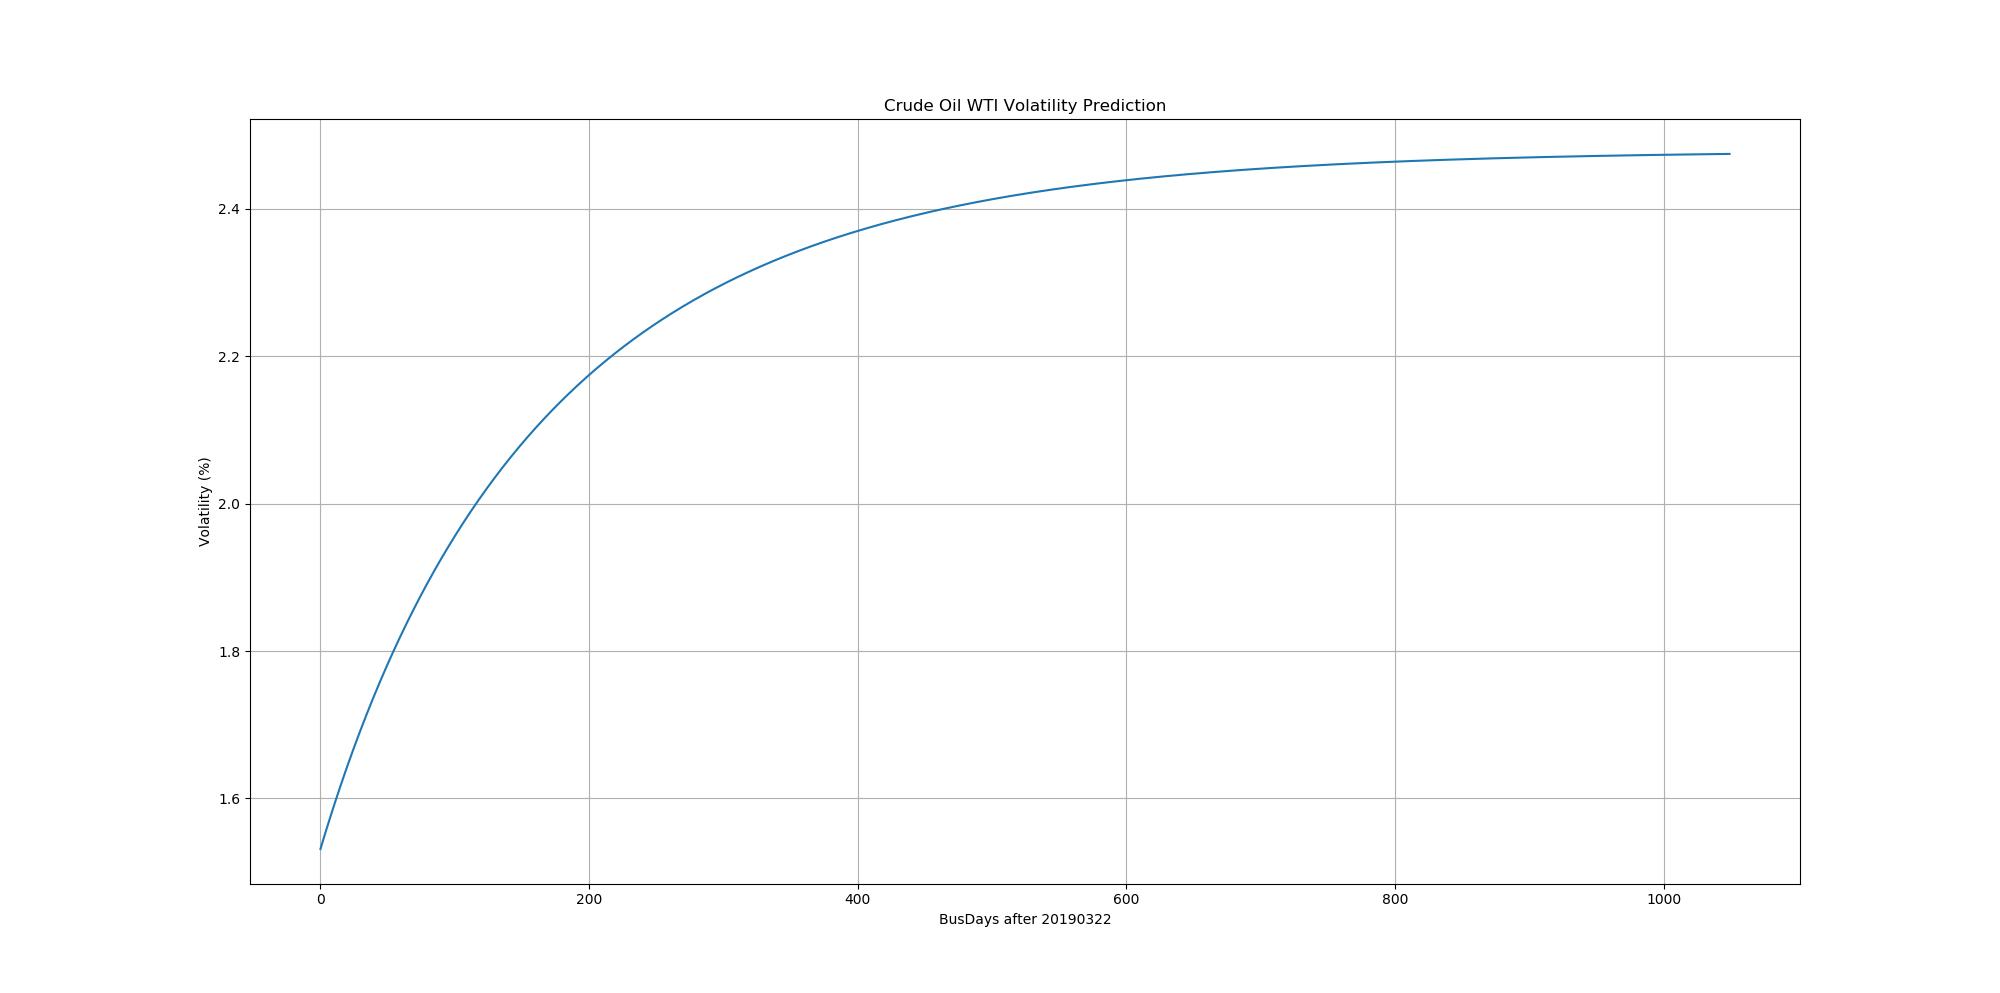
\includegraphics[width=\linewidth]{CrudeOilvol.png} % Figure image
	\caption{Volatility Prediction on Crude Oil} % Figure caption
	\label{oil pred} % Label for referencing with \ref{bear}
\end{figure}

\begin{figure}[!ht]
	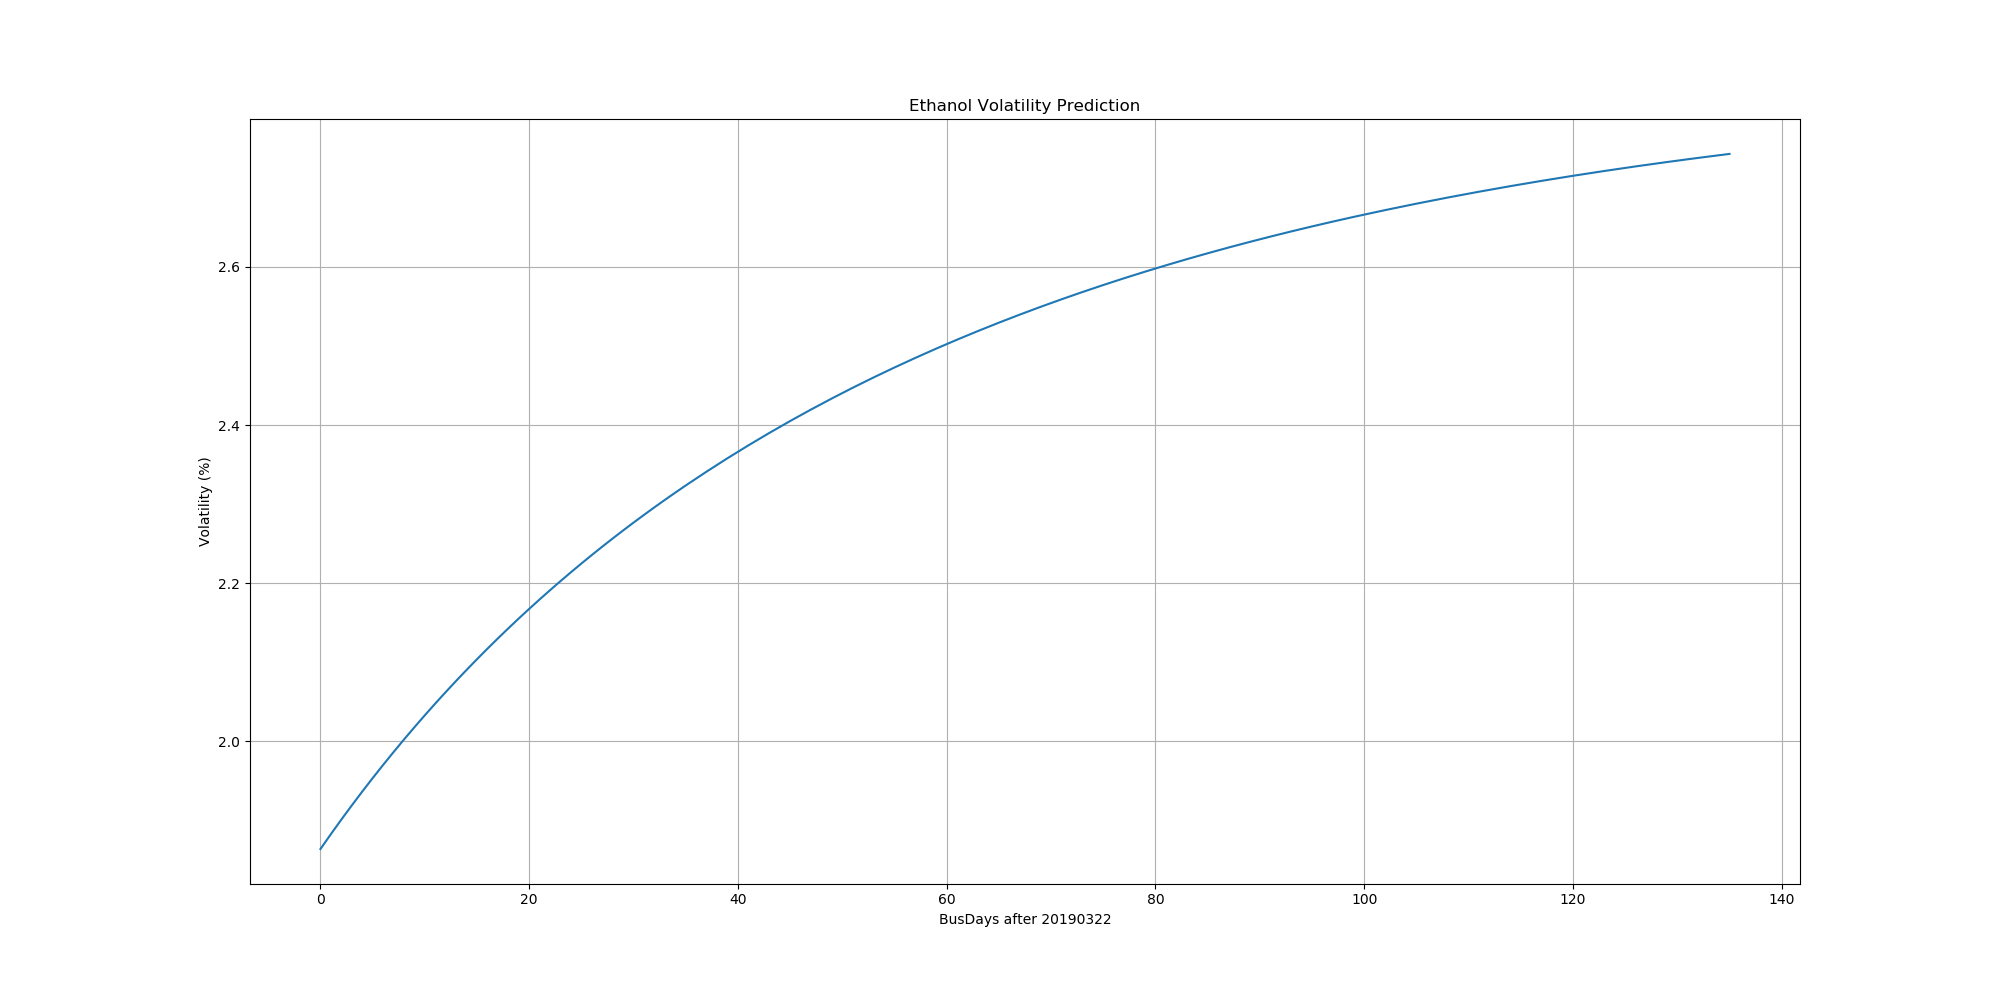
\includegraphics[width=\linewidth]{Ethanolvol.png} % Figure image
	\caption{Volatility Prediction on Ethanol} % Figure caption
	\label{eth pred} % Label for referencing with \ref{bear}
\end{figure}

\begin{figure}[!ht]
	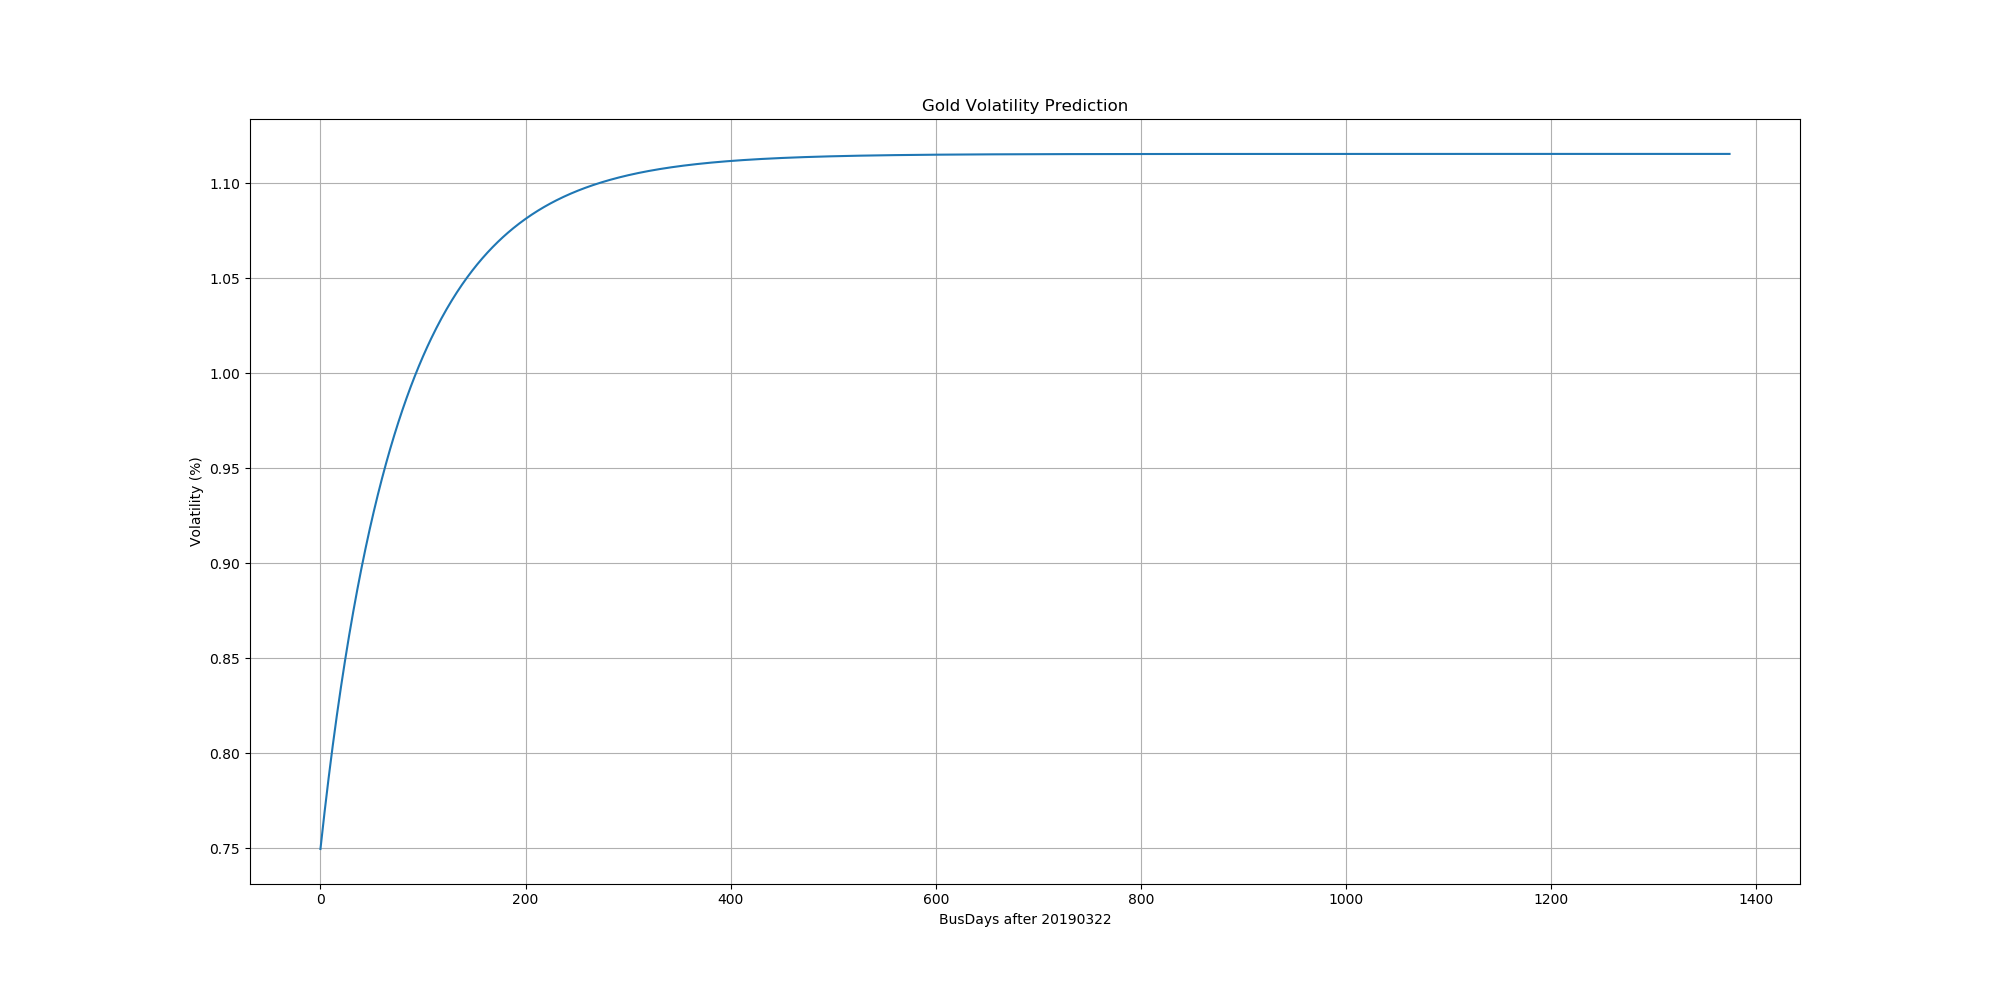
\includegraphics[width=\linewidth]{Goldvol.png} % Figure image
	\caption{Volatility Prediction on Gold} % Figure caption
	\label{gold pred} % Label for referencing with \ref{bear}
\end{figure}

\begin{figure}[!ht]
	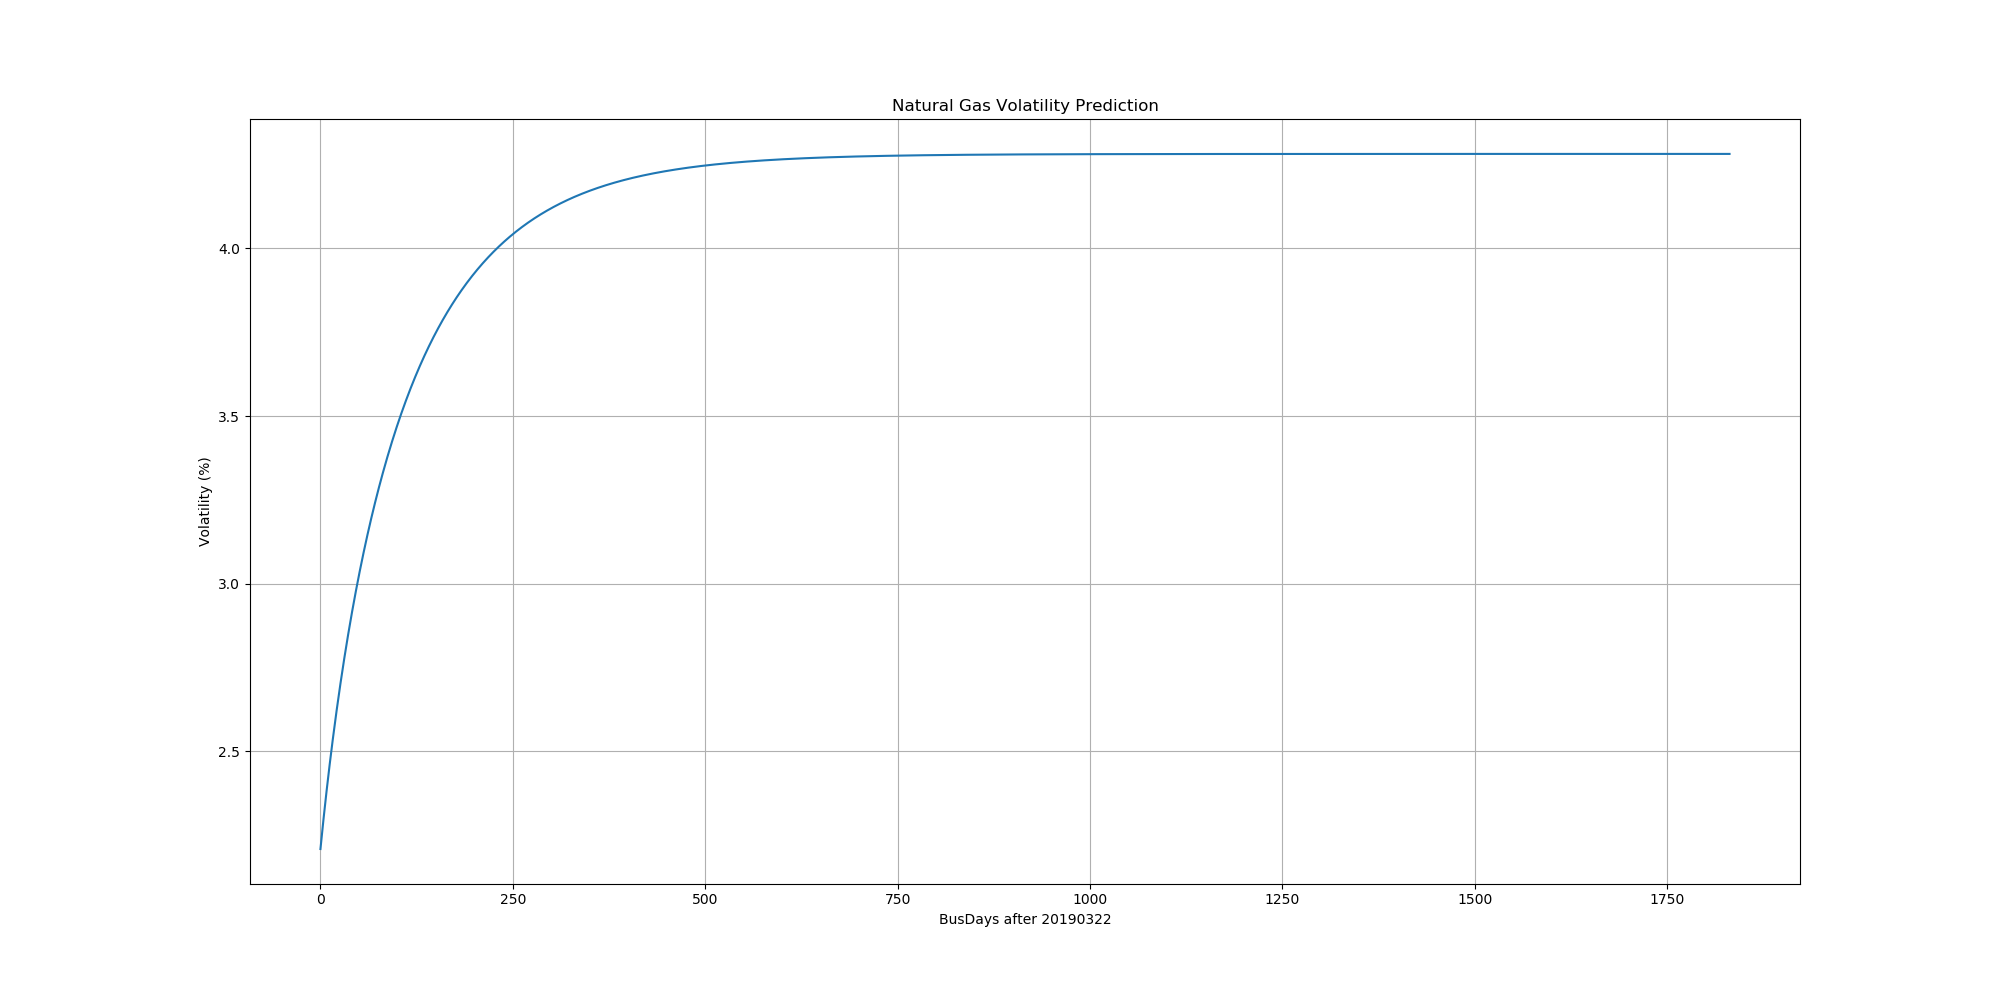
\includegraphics[width=\linewidth]{Naturalgasvol.png} % Figure image
	\caption{Volatility Prediction on Natural Gas} % Figure caption
	\label{gas pred} % Label for referencing with \ref{bear}
\end{figure}

\begin{figure}[!ht]
	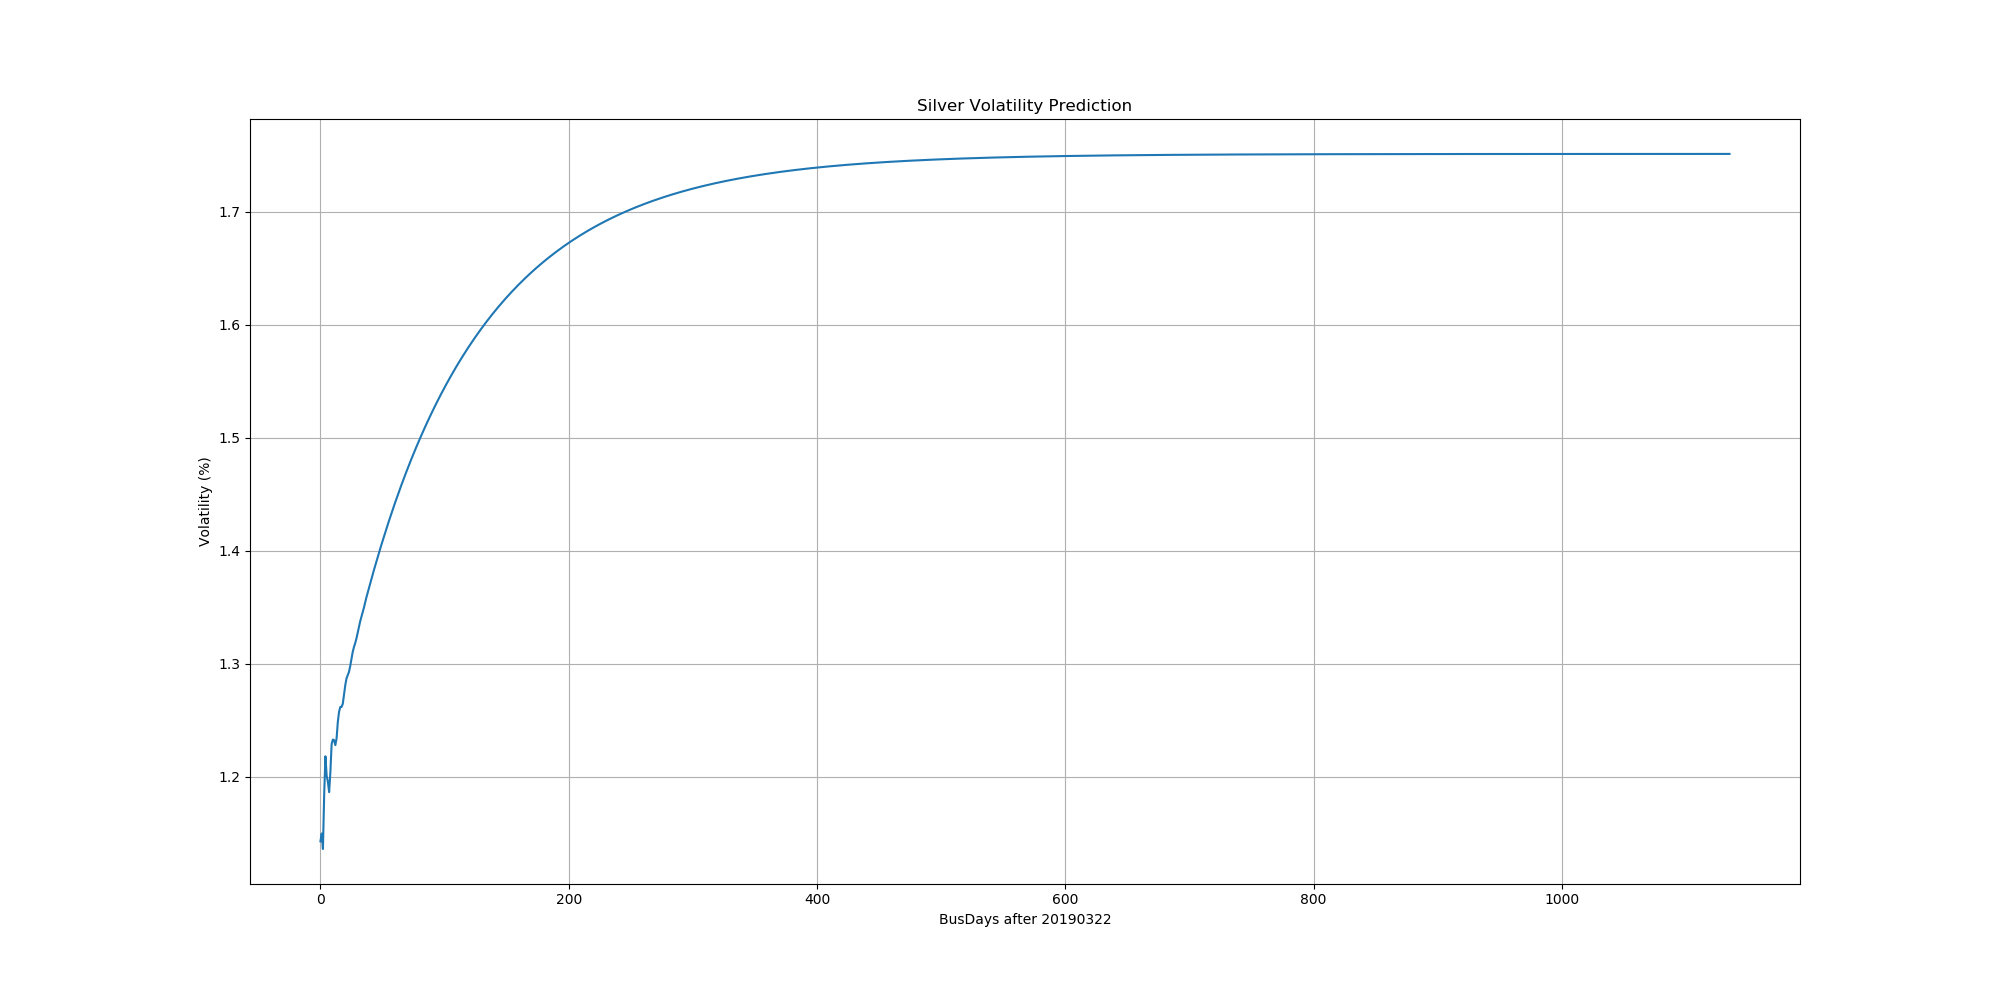
\includegraphics[width=\linewidth]{Silvervol.png} % Figure image
	\caption{Volatility Prediction on Silver} % Figure caption
	\label{silver pred} % Label for referencing with \ref{bear}
\end{figure}


\clearpage

\subsection{Tables}
\begin{table}[!ht]
	\centering
	\footnotesize
	\begin{tabular}{lcccccccccc}
		\toprule
		\multirow{2}{*}{Models}  & \multicolumn{2}{c}{Crude Oil WTI} & \multicolumn{2}{c}{Ethanol} & \multicolumn{2}{c}{Gold} & \multicolumn{2}{c}{Silver} & \multicolumn{2}{c}{Natural gas} \\
		& put & call & put & call & put & call & put & call & put & call  \\
		\midrule
		GARCH-MC & 46.679 & 304.798 & 10.757 & 25.258 & 72.799 & 84.586 & 17.455 & 26.597 & 215.232 & 324.858 \\ 
		MC & 83.121 & 122.238 & 56.035 & 73.732 & 52.874 & 91.129 & 64.379 & 89.397 & 64.891 & 84.962 \\
		BT & 402.088 & 819.106 & 45.110 & 62.466 & 106.801 & 149.124 & 83.969 & 107.557 & 264.242 & 72.697 \\
		\bottomrule
	\end{tabular}
	\caption{ARE for the Asian put ans call option for each underlying futures.}
	\label{are stat}
\end{table}

\clearpage
\subsection{Scripts}

\subsubsection{corr.py}
\lstinputlisting{corr.py}

\subsubsection{binomialTreePrice.py}
\lstinputlisting{binomialTreePricer.py}

\subsubsection{biTreePriceSimulation.py}
\lstinputlisting{biTreePriceSimulation.py}

\subsubsection{garchPricer.py}
\lstinputlisting{garchPricer.py}



\end{document}
